%    \red{Measurement of the magnitude of the collected charge has also been generally available for pixel detectors, and has been used to improve the 3D space point precision through interpolation as well as for particle identification through specific ionization measurement.
\red{\begin{itemize}
    \item rifai il conto della lunghezza di attenuazione. Ho trovato (presentazione Luciano Mus) 29 um per ka e 37 um per kb. 
    \item Con il PMOS la configurazione del FE di default è: e richiama i significati delle variabili. 
    \item parla dell HV
\end{itemize}}

\section{TJ-Monopix1 characterization}
    \subsection{Threshold and noise: figure of merit for pixel detectors}
        %python3 -i calibration/scurve_tot_histo.py -f calibration/calibration_data/20220506 -i 1 100 questo script crea i file di output contenenti i gli istogrammi del tot e della s curve
        %python3 -i calibration/tot_charge_plotting.py -f calibration/calibration_data/20220506 per fare il plot della s curve e relativi residui 
        %python3 -i calibration/tot_histo2d.py -f calibration/calibration_data/PMOS/20220506 per fare l'istogramma 2d del tot           
        A characterization of threshold and noise is typically necessary since these values have an impact on the operating conditions and on the performance of the chips, so much that the signal to threshold ratio may be considered as the figure of merit for pixel detectors rather than the signal to noise ratio.
        The mean minimum stable threshold evolved through different generation of chips: in the 1st generation it was around \SI{2500}{e-} while in the 3rd (corresponding to nowadays chips) is less than \SI{500}{e-}. This allows in thinner sensors with smaller signals: from \SI{16000}{e-} produced in \SI{200}{\um}, the signal expected moved down to \SI{2000}{e-} produced in \SI{25}{\um}. According with this, the threshold of TJ-Monopix1 is around \SI{500}{e-}.
 
        Obviously the threshold has to be located between the noise peak around the baseline and the signal distribution, in particular it has to be low enough to mantain a high signal efficiency, but also high enough to cut the noise: for a low threshold many pixels can fire at the same time and a positive feedback can set off a chain reaction eventually, causing all the other pixels to fire.
        Thus, the noise sets a lower bound to the threshold: if an occupancy $\leqslant$ $10^{-4}$ is required, for example, this correspond to the Gaussian 1-sided tail fraction for \SI{3.7}{\sigma}.
        In this case, if the noise is \SI{100}{e-} (resonable), the threshold must be higher than \SI[parse-numbers=false]{3.7\times100}{e-}.
        Typically this argument sets only a minimal bound to the threshold since the variation with time and from pixel to pixel have to be taken into account: the temperature, the anealing (for example, the radiation damages in the oxide layer causes shift of MOSFET threshold voltage) and the process parameters variation across the wafer (as for example process mismatch between transistors). 

        
        Given that the first stage of amplification is the most crucial, since in the following stages the signal amplitude is high compared to additional noise, the noise is valued at the preamplifier input node.
        Then, the noise is parameterized as Equivalent Noise Charge (ENC), which is defined as the ratio between the noise N at the output expressed in Volt and the out voltage signal S produced by \SI{1}{e-} entering in the preamplifier:
        \begin{equation}
            ENC\, =\, \frac{N_{out}[V]}{S_{out}[V/e-]}\,=\,\frac{V^{RMS} _{noise}}{G}
        \end{equation} 
        with G expressed in \si{V/e-}; as the gain increases, the noise reduces . 
        \red{Servirebbe una misura}

        Considering the threshold dispersion a requirement for the ENC is: 
        \begin{equation}
            ENC < \sqrt{(T/3.7)^2 - T_{RMS} ^2 (x) - T_{RMS} ^2 (t)}
        \end{equation}
        where the T is the threshold setted, $T_{RMS}$ is the threshold variation during time (t) and across the matrix (x); a typical reasonable value often chosen is \SI{5}{ENC}.

        Because of the changing of the 'real' threshold, the possibility of changing and adapting the setting parameters of the FE, both in time and in space is desiderable: these parameters are usually set by Digital to Analog Converter (DAC) with a number of bit in a typical range of 3-7.
        Unfortunately DAC elements require a lot of space that may be not enough on the pixel area; therefore, the FE parameters are typically global, which means that they are assigned for the whole chip, or they can be assigned for regions the matrix is divided into. 
        The former case corresponds to TJ-Monopix1's design in which 7 bits are used for a total 127-DAC possible values, while the latter corresponds to the ARCADIA-MD1's one, \red{where quanti bit??}. 
        An other possibility, for example implemented in TJ-Monopix2, is allocate the space on each pixel for a subset of bits, then combinig the global threshold with a fine tuning. 
        If so, the threshold dispersion after tuning is expected to be inversely proportional to the tuning DAC number of bits and thus be improved a lot:
        \begin{equation}
            \sigma_{THR, tuned} = \frac{\sigma_{THR}}{2^{n bit}}
        \end{equation}    
        where $\sigma_{thr}$ 
        is the RMS of the threshold spread before tuning.

        To measure the threshold and noise of pixels a possible way is to make a scan with different known injected charge: the threshold corresponds to the value where the efficiency of the signal exceeds the 50\%, and the ENC is determined from the width of this edge.        
        Following this path, I have used the injection circuit available on the chip to inject 100 pulses for each input charge for a fixed threshold.
        The injection comes on a capacity at the input of the FE circuit, whose mean value is \SI{230}{aF} and from which the conversion factor from DAC units to electrons can be obtained: for the PMOS flavor, for example, since the DAC are biased at \SI{1.8}{V}, the Least significant Bit (LSB) corresponds to a voltage of \SI{14.7}{mV} from which the charge for LSB \SI{1.43}{e-/mV} and the conversion factor therefore is \SI{20.3}{e-/DAC}.     
        While this value is equivalent for all the PMOS flavor, the HV flavor is expected to have a different conversion factor, $\sim$ \SI{33}{e-/DAC}, beacuse of the different input capacity. 

        Besides the charge, also the duration and the period of the injection pulse can be set; it is important to make the duration short enough to have the falling edge during thed dead time of the pixel (in particular during the FREEZE signal) in order to avoid the undershoot, coming at high input charge, triggering the readout and reading spurious hits. 
        Since the injection circuit is coupled in AC to the FE, if the falling edge of the pulse is sharp enought to produce ad undershoot, this can be seen as a signal. 

        \begin{figure}[h!]
            \centering
            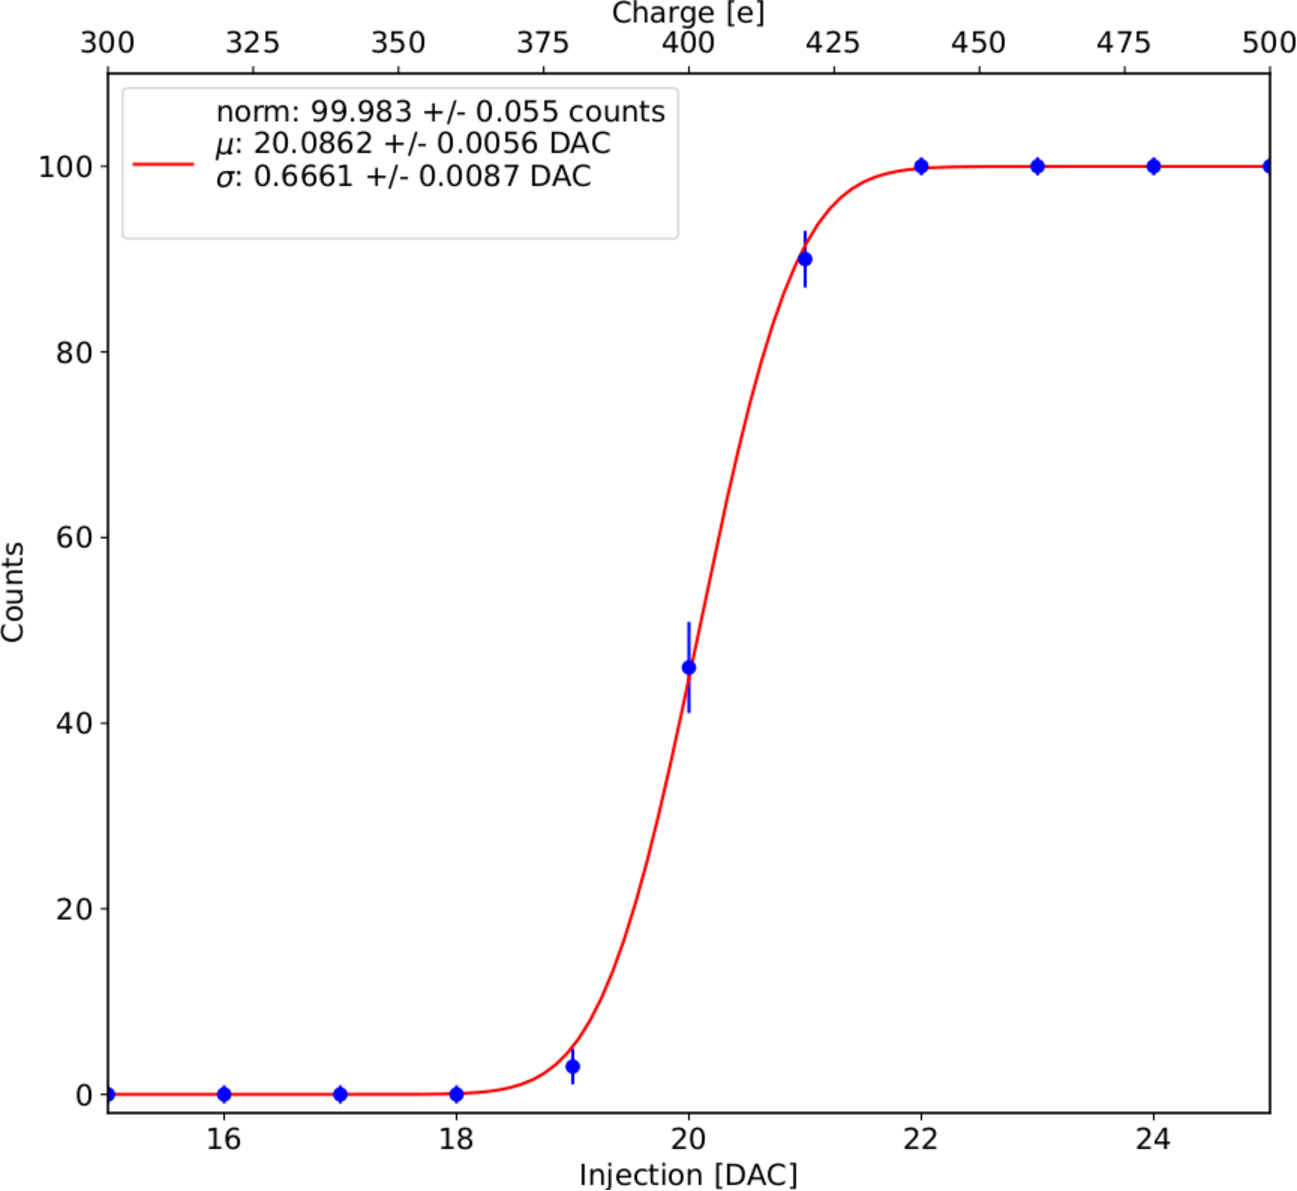
\includegraphics[width=.6\linewidth]{figures/charaterization/scurve.pdf}
            \caption{S-curve for pixel (10, 10) of the PMOS flavor (flavor 1) with IDB fixed at \SI{40}{DAC}. The conversion of charge injected from DAC to electrons has been done assuming a conversion factor of \SI{20}{e-/DAC}. }
            \label{fig:scurve}
        \end{figure}   
        Assuming a gaussian noise, the efficiency of detecting the signal can be described through a modification of the error function:
        \begin{equation}
            f(x, \mu, \sigma) = \frac{1}{2} \; \left(1\,+\,erf\left(\frac{x-\mu}{\sigma \sqrt{2}}\right)\right)
            \label{eq:fit_scurve}
        \end{equation}
        \red{with:} 
        %\begin{equation} 
        %    erf(z) = \[ \int_{0}^{z} \frac{2}{\sqrt{\pi}} e^{-x^2} dx  \]
        %\end{equation} 
        where the threshold and the ENC corresponds to the $\mu$ and $\sigma$.
        Therefore I perform a fit of the counts detected using the function in equation \ref{eq:fit_scurve}. In figure \ref{fig:scurve} there is an example with IDB equal to \SI{40}{DAC} of fit for a pixel belonging to the flavor B, while in table \ref{tab:Flavor_PMOS_reser} and figure \ref{fig:threshold_noise_hist} there are the histograms and the maps of the parameters of the scurve-fit. As expected, the flavor PMOS reset gated (A), thanks to the transistor which change the baseline value, has a lower threshold and noise
        \begin{figure}[h!]
            \centering
            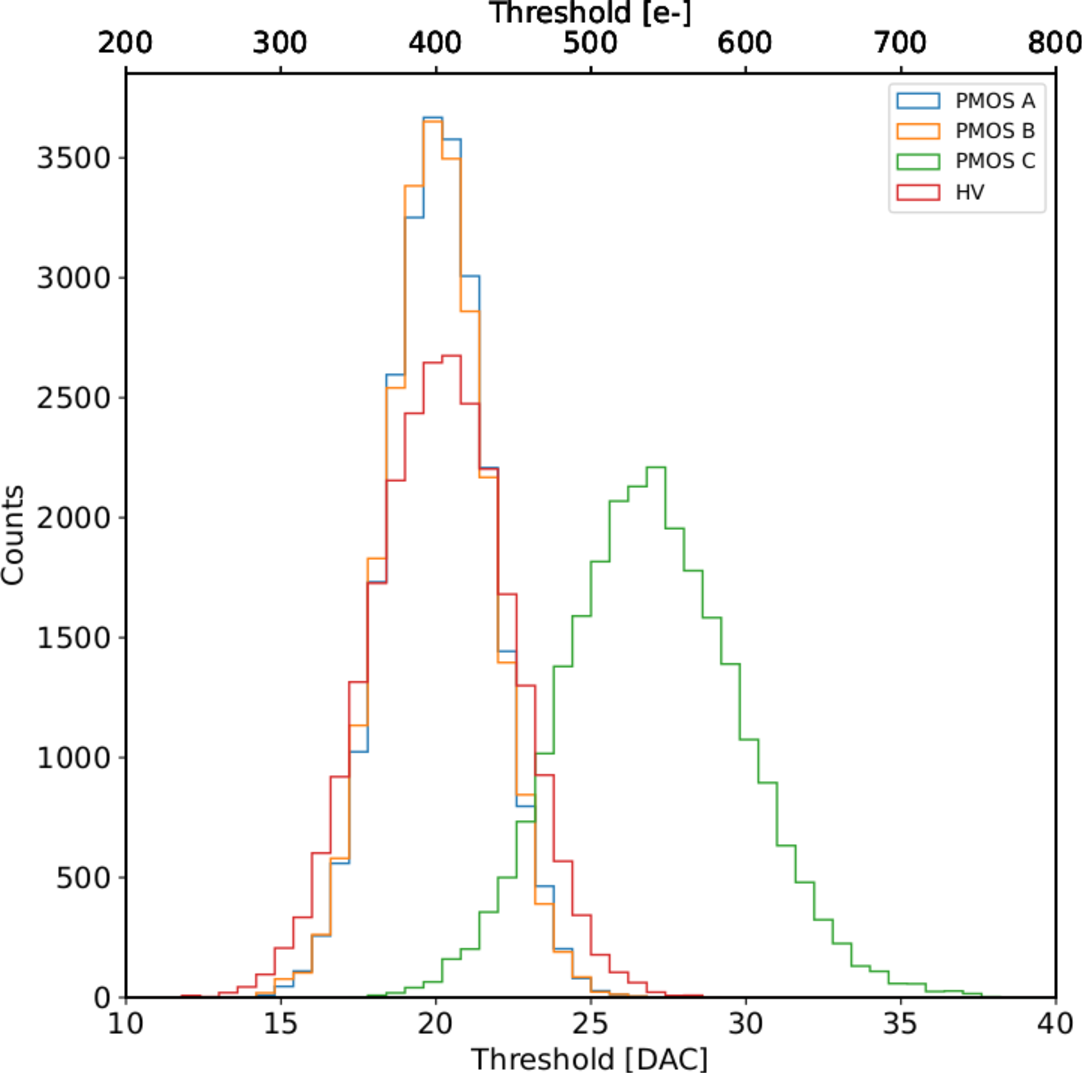
\includegraphics[width=.49\linewidth]{figures/charaterization/threshold_histogram.pdf}
            \includegraphics[width=.49\linewidth]{figures/charaterization/noise_histogram.pdf}\\
            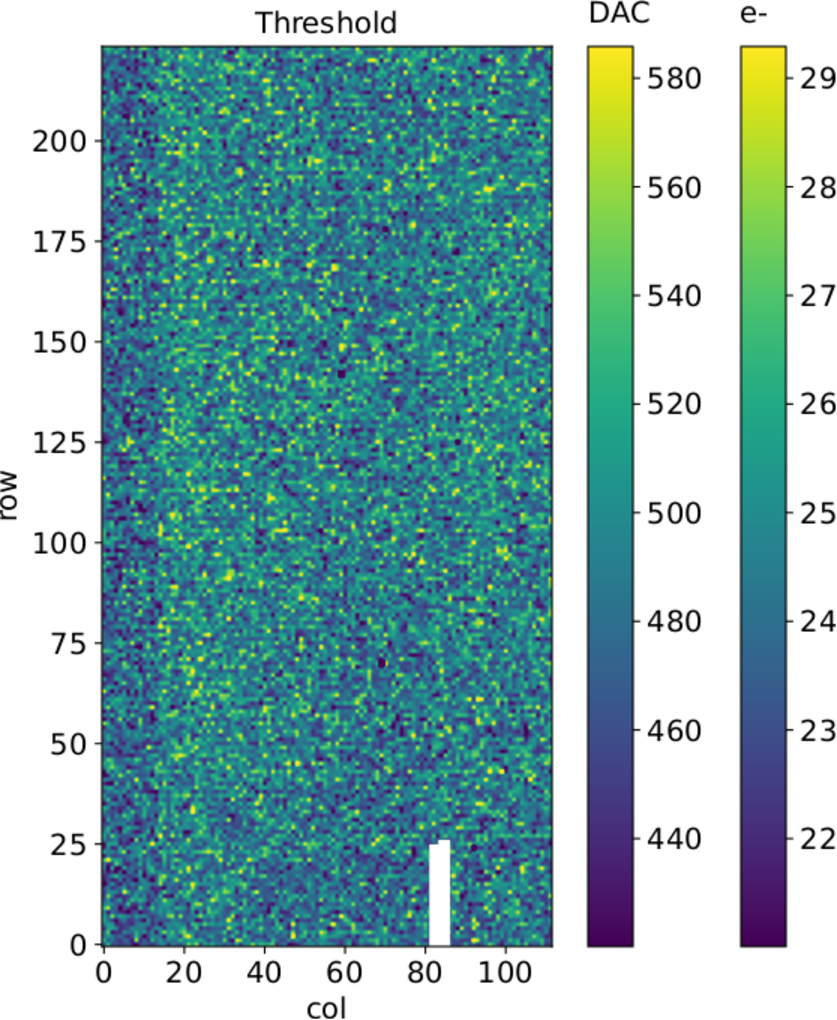
\includegraphics[width=.49\linewidth]{figures/charaterization/threshold_map.pdf}
            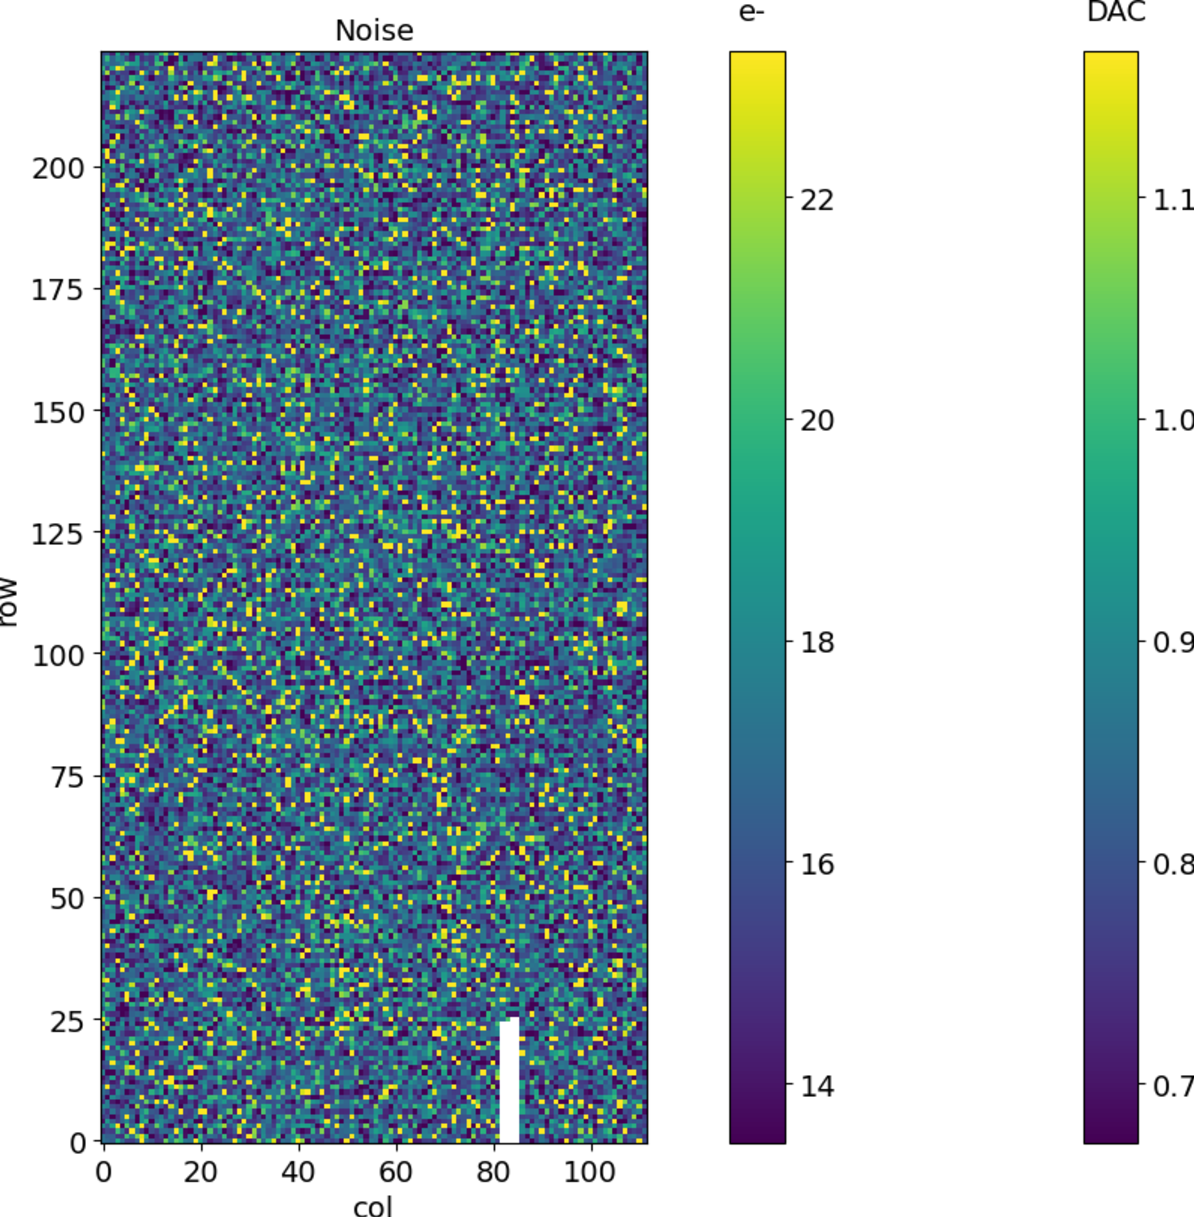
\includegraphics[width=.49\linewidth]{figures/charaterization/noise_map.pdf}            
            \label{fig:threshold_noise_hist}
            \caption{Histograms of the threshold (a) and the noise (b) found fitting the s-curve of \red{all} flavor with IDB fixed at \SI{40}{DAC}. Below there are the maps of the threshold (a) and the noise (b), respectively, found fitting the s-curve with IDB fixed at \SI{40}{DAC} for the PMOS flavor (B). The white pixels have the injection circuit broken.}
        \end{figure}      
        %\begin{table}
        %        \begin{center}
        %        \begin{tabular}{| c | c | c |}
        %        \hline
        %         & DAC units & electrons \\
        %        \hline
        %        \hline
        %        Threshold        & 24.529 $\pm$ 0.049 & 511.0 $\pm$ 1.0 \\
        %        Threshold dispersion & 1.848 $\pm$ 0.033 & 36.96$\pm$0.66\\
        %        Noise            & 0.8222 $\pm$ 0.0043 & 16.444$\pm$0.086 \\
        %        Noise dispersion & 0.0975 $\pm$ 0.0030 & 1.95$\pm$0.06\\
        %        \hline
        %        \end{tabular}
        %        \caption{Flavor PMOS, IDB fixed at \SI{40}{DAC}}
        %        \label{tab:Flavor_PMOS_reser}
        %        \end{center}
        %\end{table}        

        \begin{table}
            \begin{center}
            \begin{tabular}{| c |  c | c | c |c |}
            \hline
            & PMOS A & PMOS B & PMOS C & HV \\
            \hline
            \hline
            Threshold [\si{e-}] & &\\
            Threshold dispersion [\si{e-}] &  &\\
            Noise [\si{e-}] &  &\\
            Noise dispersion [\si{e-}] & &\\
            \hline
            \end{tabular}
            \caption{Mean threshold and noise parameters for \red{all} flavor and their dispersion on the matrix. }
            \label{tab:calibration_param}
            \end{center}
        \end{table}       

    
        %Furthermore the two portion of the chip, with FDPW and with RDPW, have been analyzed separately, because a small difference in the sensor input capacitance was expected: in fact, the deep p-well removal in the RDPW causes a small reduction of the depletion region around the collection electrode, which results in an increase of the sensor capacitance C.
        %\red{Then  , the charge to voltage conversion gain at the front-end input (Q /C ) is lower and as a result, for the same input charge a lower voltage amplitude is induced at the front-end input. }
    
    
        Small threshold variations has been observed in the first biasing section (columns from 0 to 14) with IDB=\SI{40}{DAC}; the same structure appears more evident at other different IDBs,as for example \SI{100}{DAC}
        \red{Plot of the average threshold per column al variare di IDB.} 
        The systematic threshold variation across the biasing group has not a known motivation, but one could certainly be the transistor mismatch of the biasing DAC registers IDB and ICASN, which both adjust the effective threshold (I recall that ICASN regulate the baseline, and in this measurements it was set to the minimin possible value).

        %GUARDA A PAGINA 127 DELLA TESI PER GLI ULTIMI DUE FLAVOR

        To verified the trend of the threshold as a function of the front end parameter IDB and find its dynamic range, I have permormed different scans changing the IDB: I have injected the whole matrix and found the means and the standard deviation of the distributions. The results are shown in figure \ref{fig:threshold_vs_IDB}: the blue points are the mean threhsold found whithin the matrix, while in green is shown the width of the threshold distribution, aka the threshold dispersion. 
        While the threshold increases, the ENC decreases of $\sim$\SI{4}{e-},which is $\sim$1/3 of the noise at IDB=\SI{40}{DAC}. 
        \begin{figure}[h!]
            \centering
            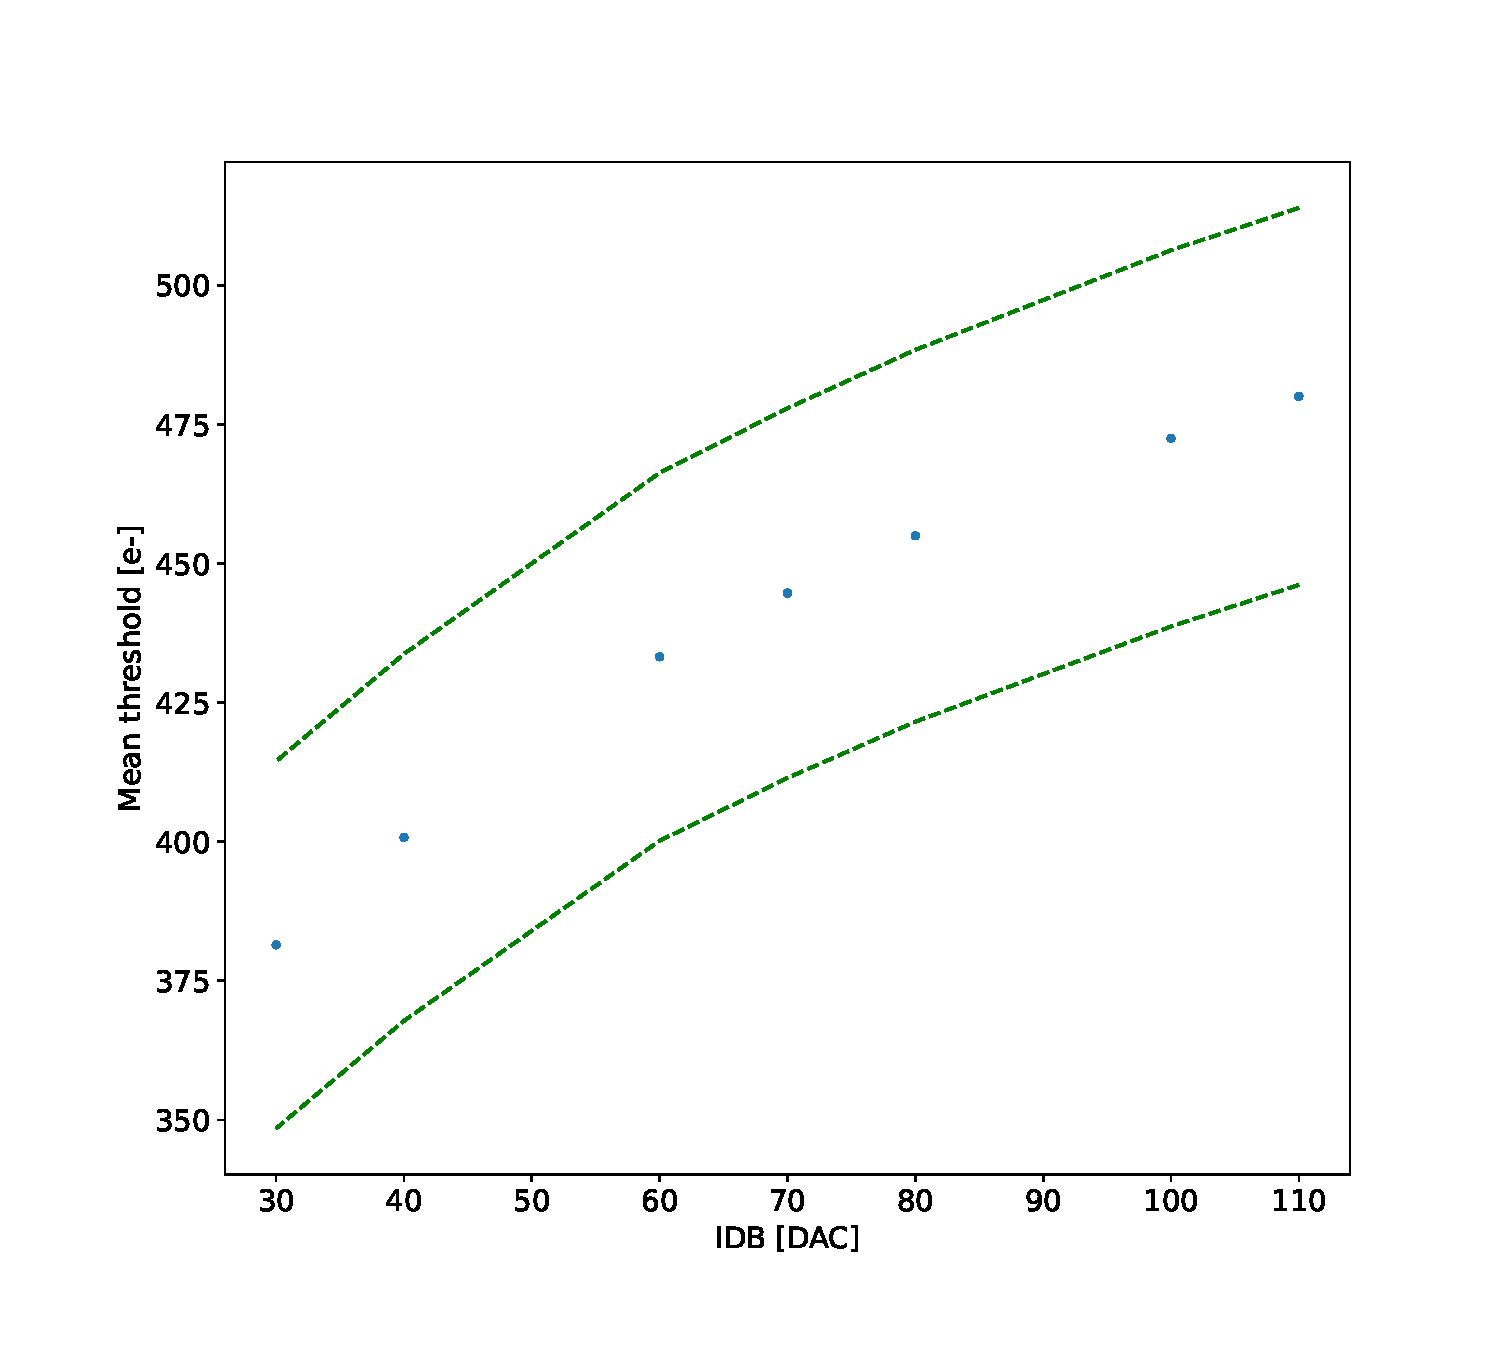
\includegraphics[width=.70\linewidth]{figures/charaterization/thr_vs_IDB.pdf}
            \caption{Flavor PMOS (B) with Psub-Pwell biased at -\SI{6}{V}.Threshold measured in electrons vs the register which sets the threshold, IDB.  }
            \label{fig:threshold_vs_IDB}
        \end{figure}            

        Then, to evaluete the operation and the occupancy of the chip at different threshold I have made long acquisitions of noise at different IDB and check how the number of pixel masked changes with the threshold. The masking algorithm I have used search for pixels with rate $>$\SI{10}{Hz} and mask them. With such algorithm, in our standard condition, IDB=\SI{40}{DAC}, a very low noise hit rate is intentionally achieved masking only \red{dozen of pixels?} of the whole flavor, and other \red{quanti} are unintentionally masked. 

    \subsection{Linearity of the ToT}    
        %python3 -i acquisition_Fe55/fit_tot_single_pixel.py -f acquisition_Fe55/source_PMOSS/ per fare il fit    
        %python3 -i acquisition_Fe55/plot_tot_single_pixel.py -f acquisition_Fe55/source_PMOSS/ -fl 'gauss_line' per fare il plot di single pixel
        I have already said in chapter \ref{chap:Monopix1} that TJ-Monopix1 returns an output signal proportional to the charge released by a particle in the epitaxial layer, which is the Time over Threshold; the ToT is saved as a 6-bit variable and then has a dynamic range equal to 0-64, which corresponds to \SIrange{0}{1.6}{\us} assuming a clock frequency of \SI{40}{MHz}.
        When a pulse is longer than \SI{1.6}{\us} the counter rolls back to zero and there is no way to distinguish that charge from a lower one with the same ToT: that is the rollover of the ToT (\ref{fig:ToT_vs_charge}(a)).   

        In order to associate the ToT (in range 0-64) to the charge, a calibration of the signal is necessary. Assuming the linearity between ToT and the charge, Q can be found: 
        \begin{equation}
            Q\, [DAC] = \frac{(ToT\,[au]\, -\, q\,[au])}{m\, [au/DAC]} 
        \end{equation}
        where m and q are the fitted parameters of the calibration.
        It is important to keep in mind that the main application target of TJ-Monopix1 is in the inner tracker detector of HEP experiments, then the main feature is the efficiency, then a rough calibration of the signal to charge is fine. The ToT information can be used both to better reconstruct the charge deposition in cluster in order to improve the track resolution, and for particle identification, especially for low momentum particles which do not reach the proper detectors.
                        
        The study of the output signal is made possibile via the injection: since the pulses are triangular, the ToT is expected to be almost linear depending on the injection charge value.
        To verify this statement and study the deviations from linearity I've fit the ToT versus the charge injected for all pixel within the matrix.
        In figure \ref{fig:ToT_vs_charge}(b) there is an example of fit for a pixel belonging to the flavor B, while in figure \ref{fig:ToT_histograms_all_fl} there are the histograms and the maps of the parameters of the line-fit for all flavors with IDB fixed at \SI{40}{DAC}. Here again a difference between biasing section appears: since the slope of the ToT is related with the gain of the preamplifier (increasing the gain also increases the ToT), the mismatch is probably due to the transistor contributing to the amplification stage.

        Before performing the fit I have calculated the mean value of the ToT of the pulses recorded for each pulse amplitude and I used the mean ToT as value for the fit. 
        The aim of the calibration obviously is finding a relation only in the range 0-64 without taking into account the rolling over hits: therefore, to prevent the rollover data from reducing the mean ToT introducing a bias in the mean value, I cut and I did not consider them. 
        If a signal bigger than the \SI{1.6}{\us} is expected in the usage of the detector, the threshold must be raised or the gain reduced, making the expected output signal in range 0-64. 
        In figure \ref{fig:ToT_vs_charge} (b) are shown both the fits with a line (red) and with a second order polynomial (green): at the bounds of the ToT range values deviate from the line model. Since the deviation is low than 1\% and it only interest the region near the 0 and the 64, in first approximation it is negligible. 
        
        \begin{figure}[h!]
            \centering
            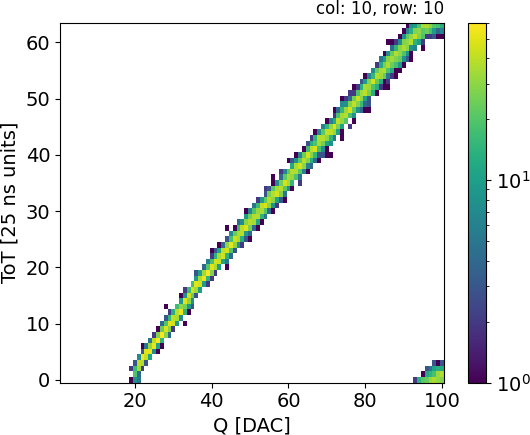
\includegraphics[width=.49\linewidth]{figures/charaterization/ToT_rollover.png}            
            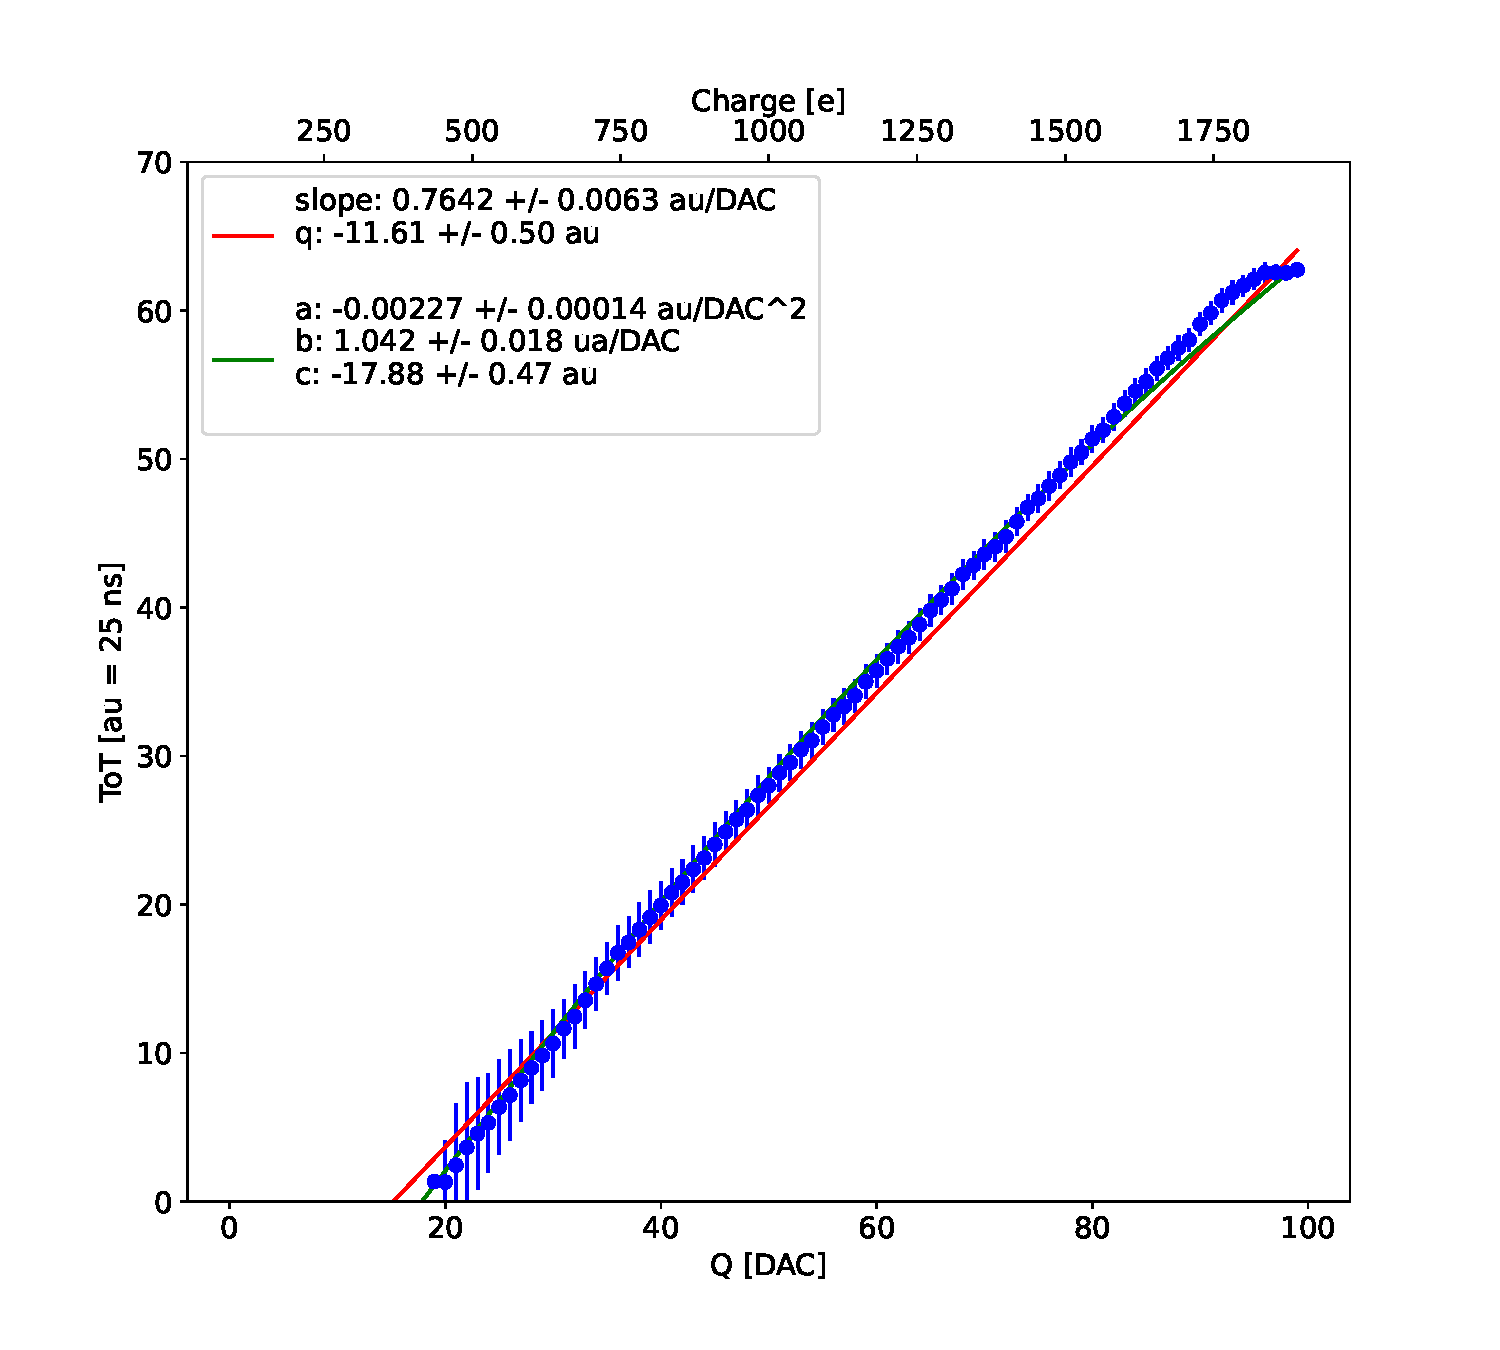
\includegraphics[width=.49\linewidth]{figures/charaterization/ToT_injection.pdf}
            \label{fig:ToT_vs_charge}
            \caption{The figures refer to pixel (10,10) of the PMOS-reset flavor (1) with IDB fixed at \SI{40}{DAC} for the PMOS flavor (B).
            (a) Histogram of the injection pulses: the ToT is in range 0-64 since it is represented by 6 bit, so when achieving the 64 it rolls over back to the zero. (b) Mean ToT vs the the charge: the mean has been calculated cutted the rolling hits. }
        \end{figure}    

        \begin{figure}[h!]
            \centering
            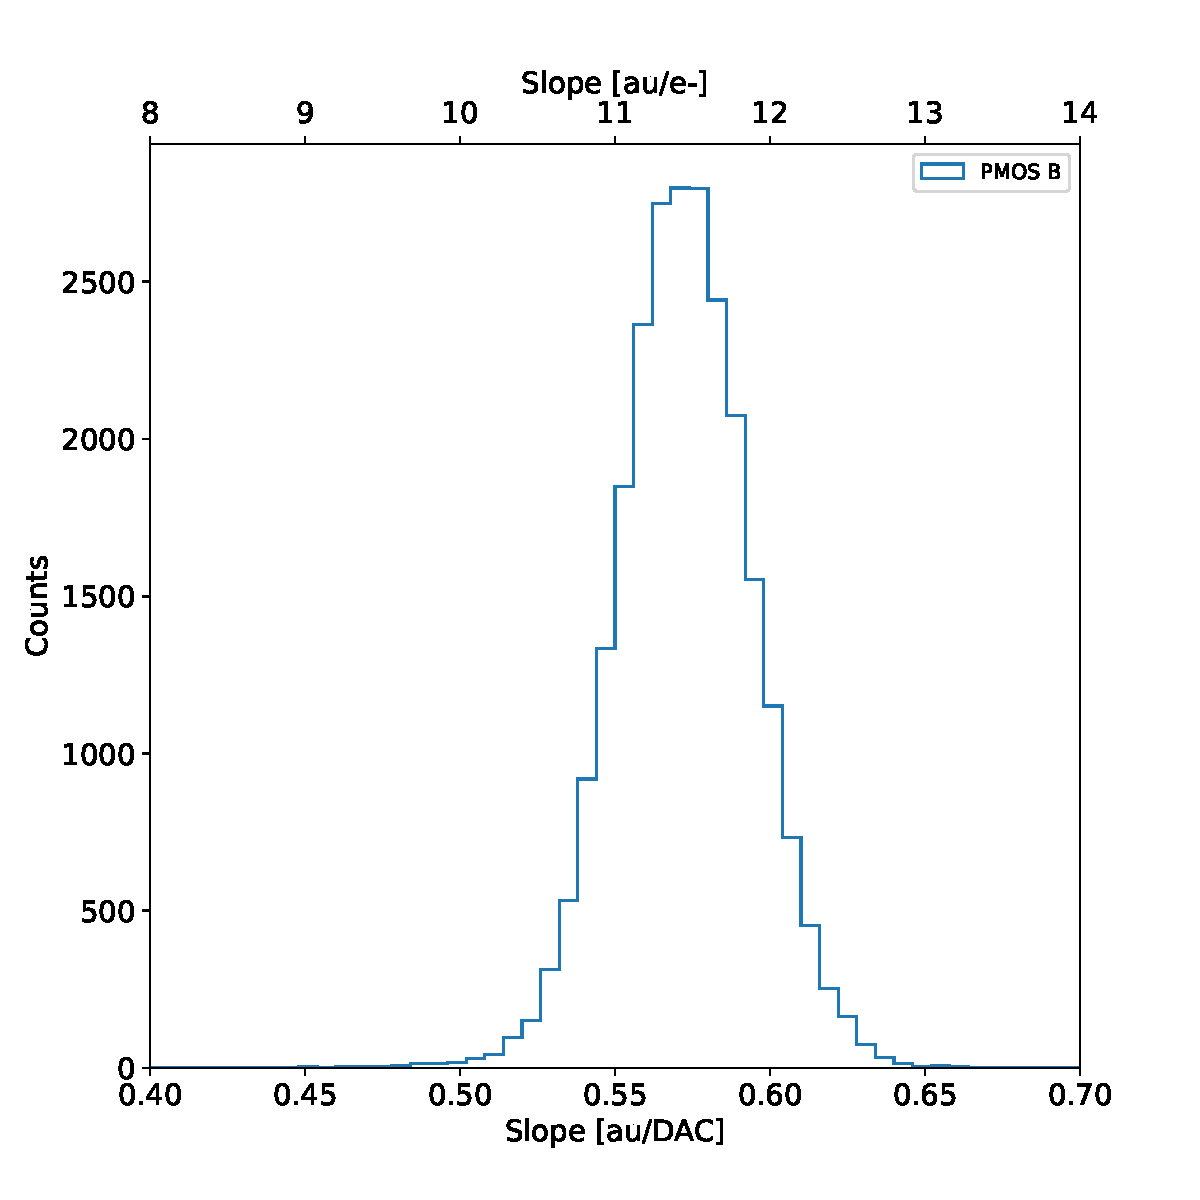
\includegraphics[width=.49\linewidth]{figures/charaterization/slope_histogram.pdf}
            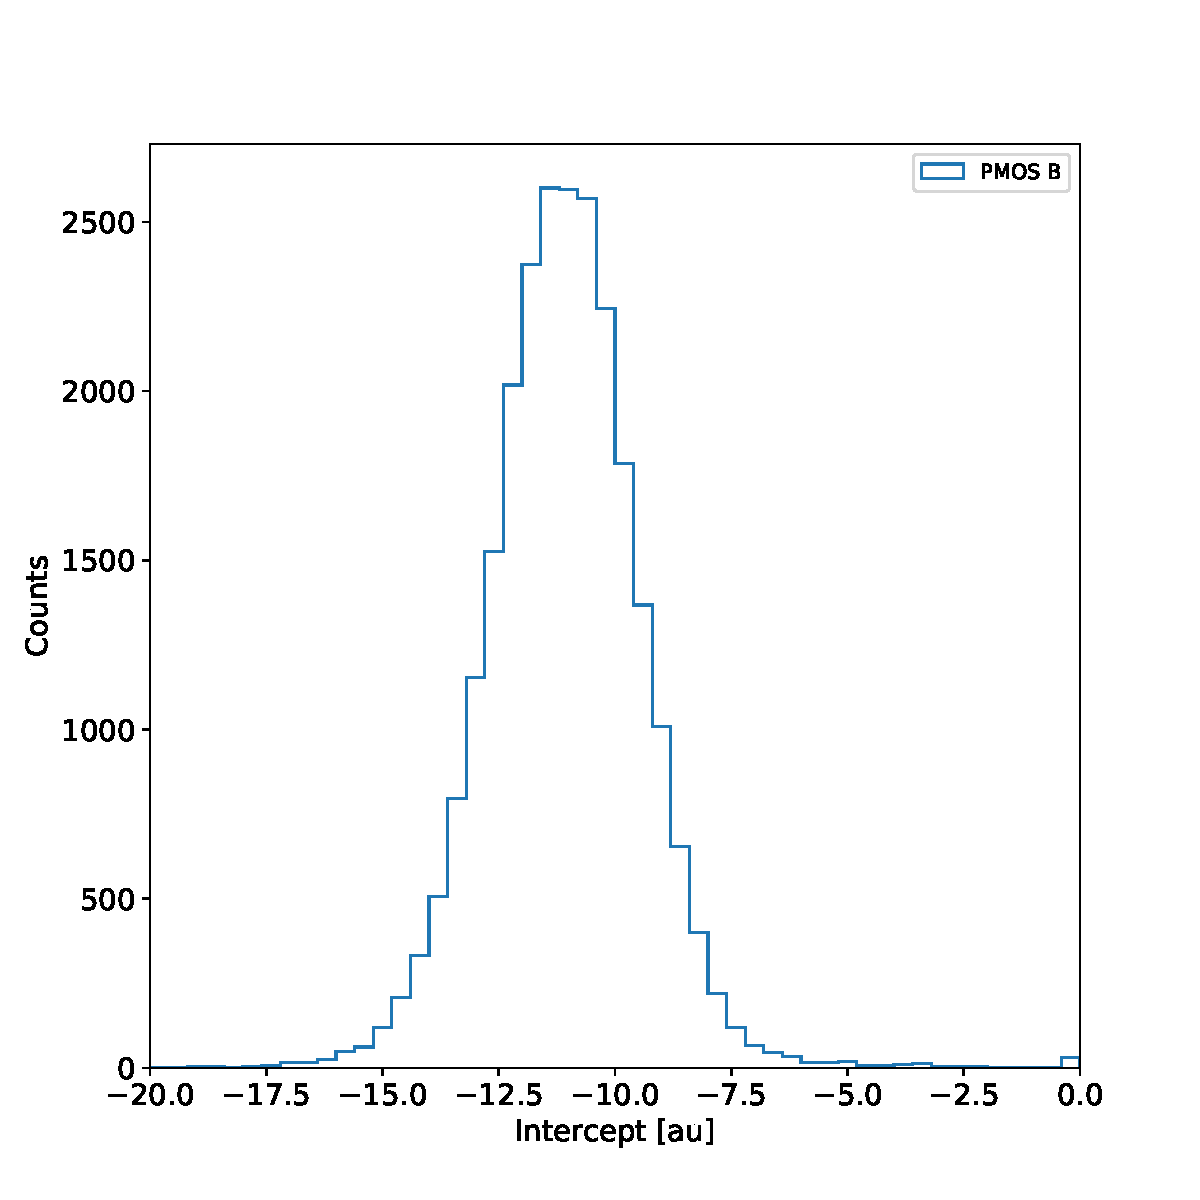
\includegraphics[width=.49\linewidth]{figures/charaterization/intercept_histogram.pdf}\\
            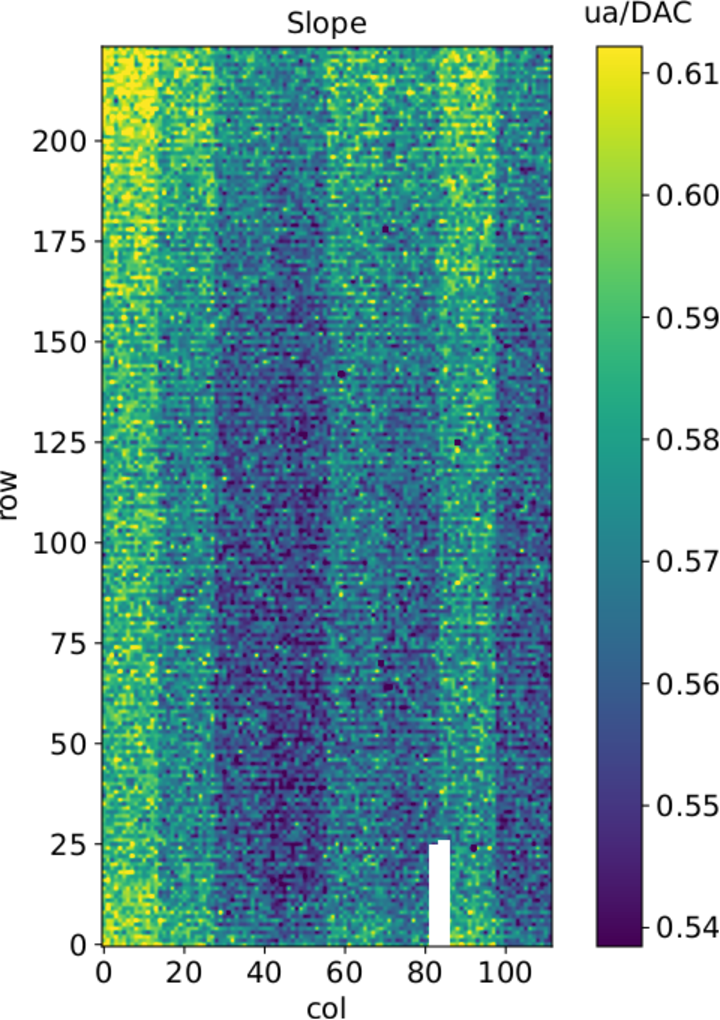
\includegraphics[width=.49\linewidth]{figures/charaterization/slope_map.pdf}
            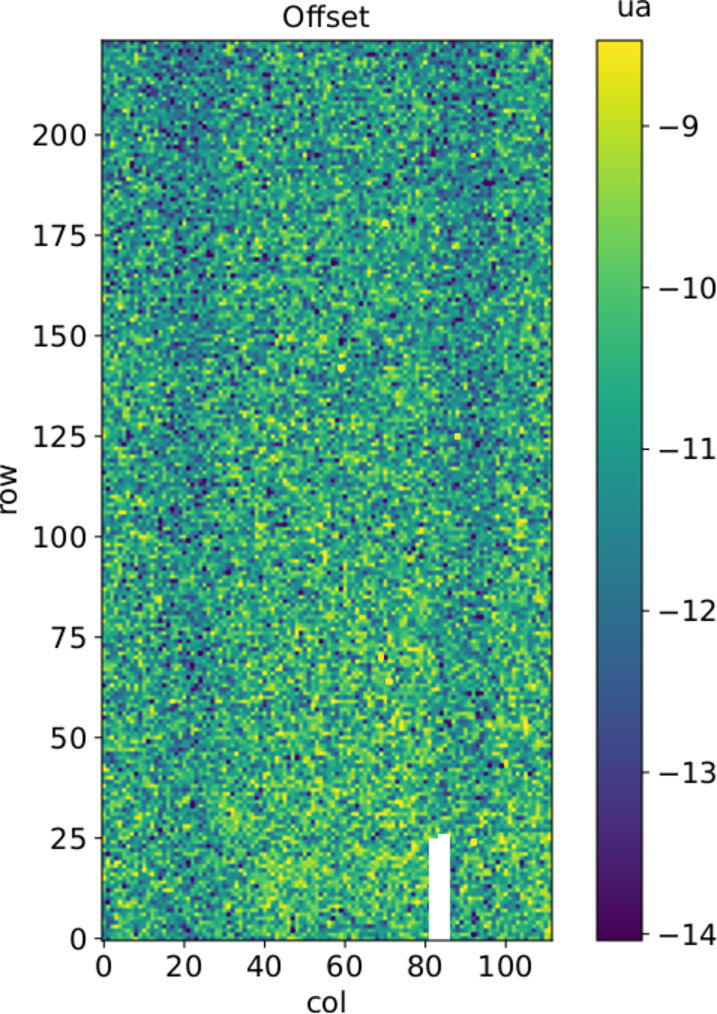
\includegraphics[width=.49\linewidth]{figures/charaterization/offset_map.pdf}
            \caption{Histograms of the calibration parameters, slope (a) and offset (b), found fitting the ToT with a line, for \red{all} flavor and with IDB fixed at \SI{40}{DAC}. Maps of the calibration parameters, slope (a) and offset (b), found fitting the ToT with a line, with IDB fixed at \SI{40}{DAC}}
            \label{fig:ToT_histograms_all_fl}
        \end{figure} 

    
    \subsection{Calibration of the ToT}
        \begin{figure}[h!]
            \centering
            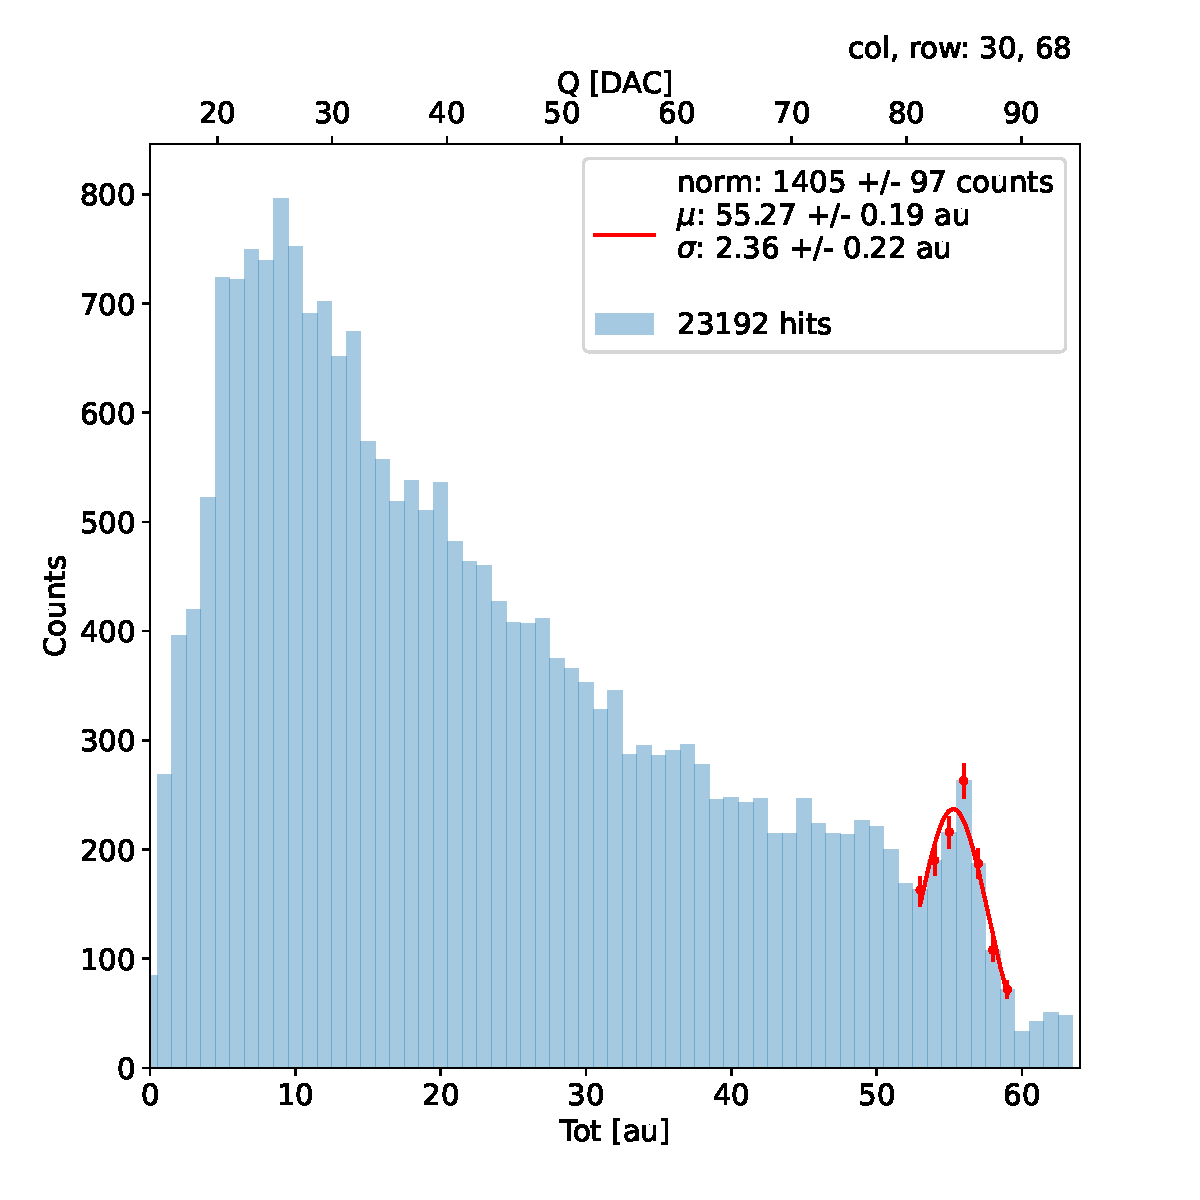
\includegraphics[width=.49\linewidth]{figures/charaterization/fit_gauss_r69.pdf}
            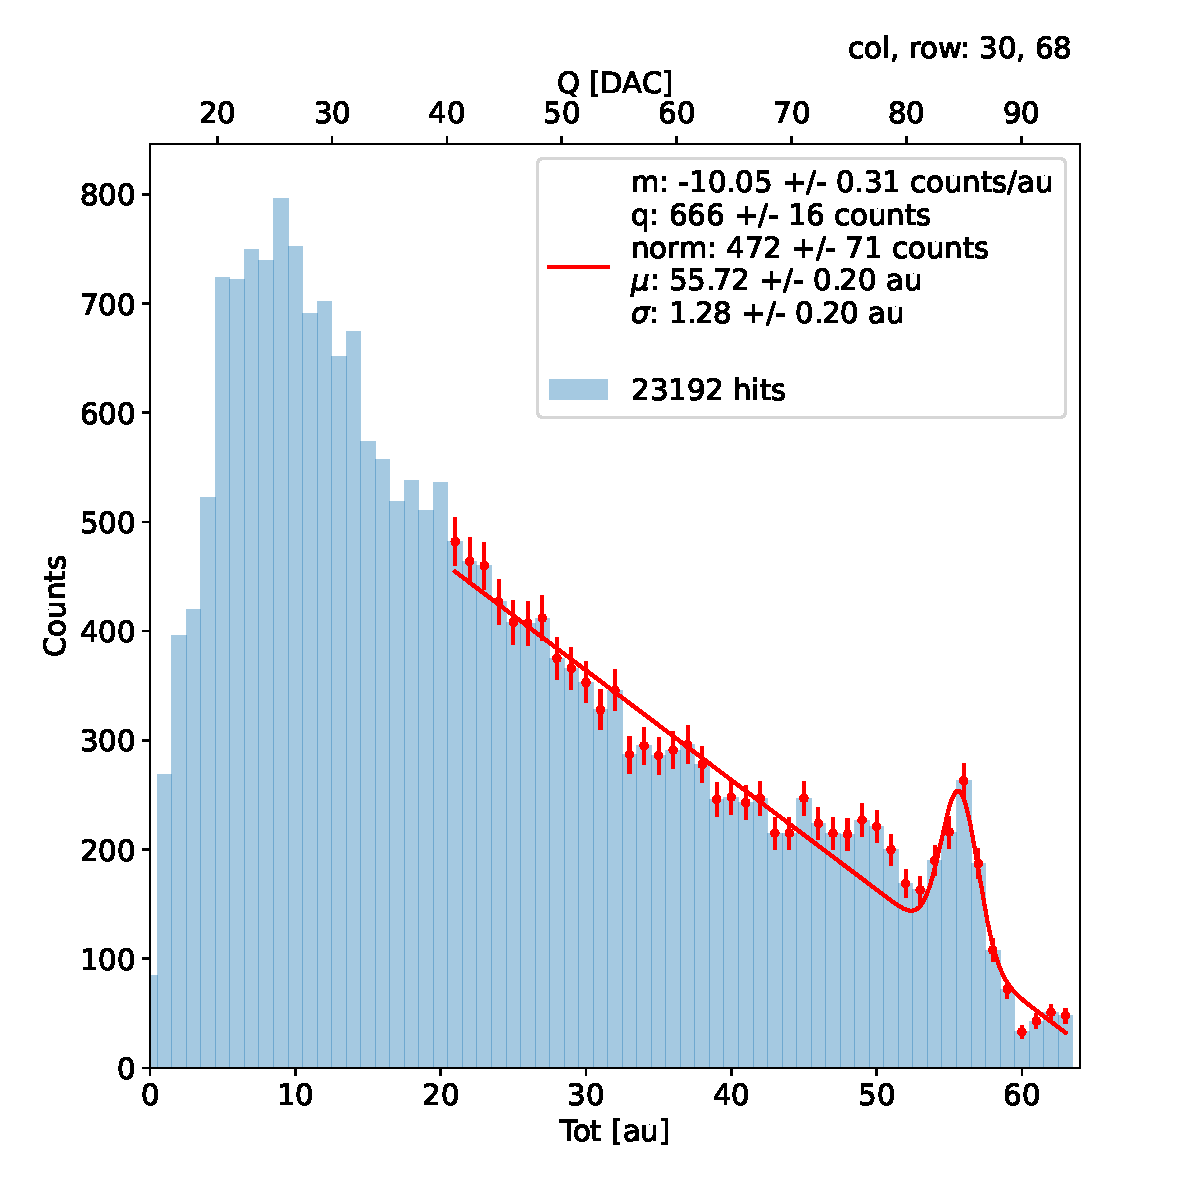
\includegraphics[width=.49\linewidth]{figures/charaterization/fit_line_gauss_r69.pdf}\\
            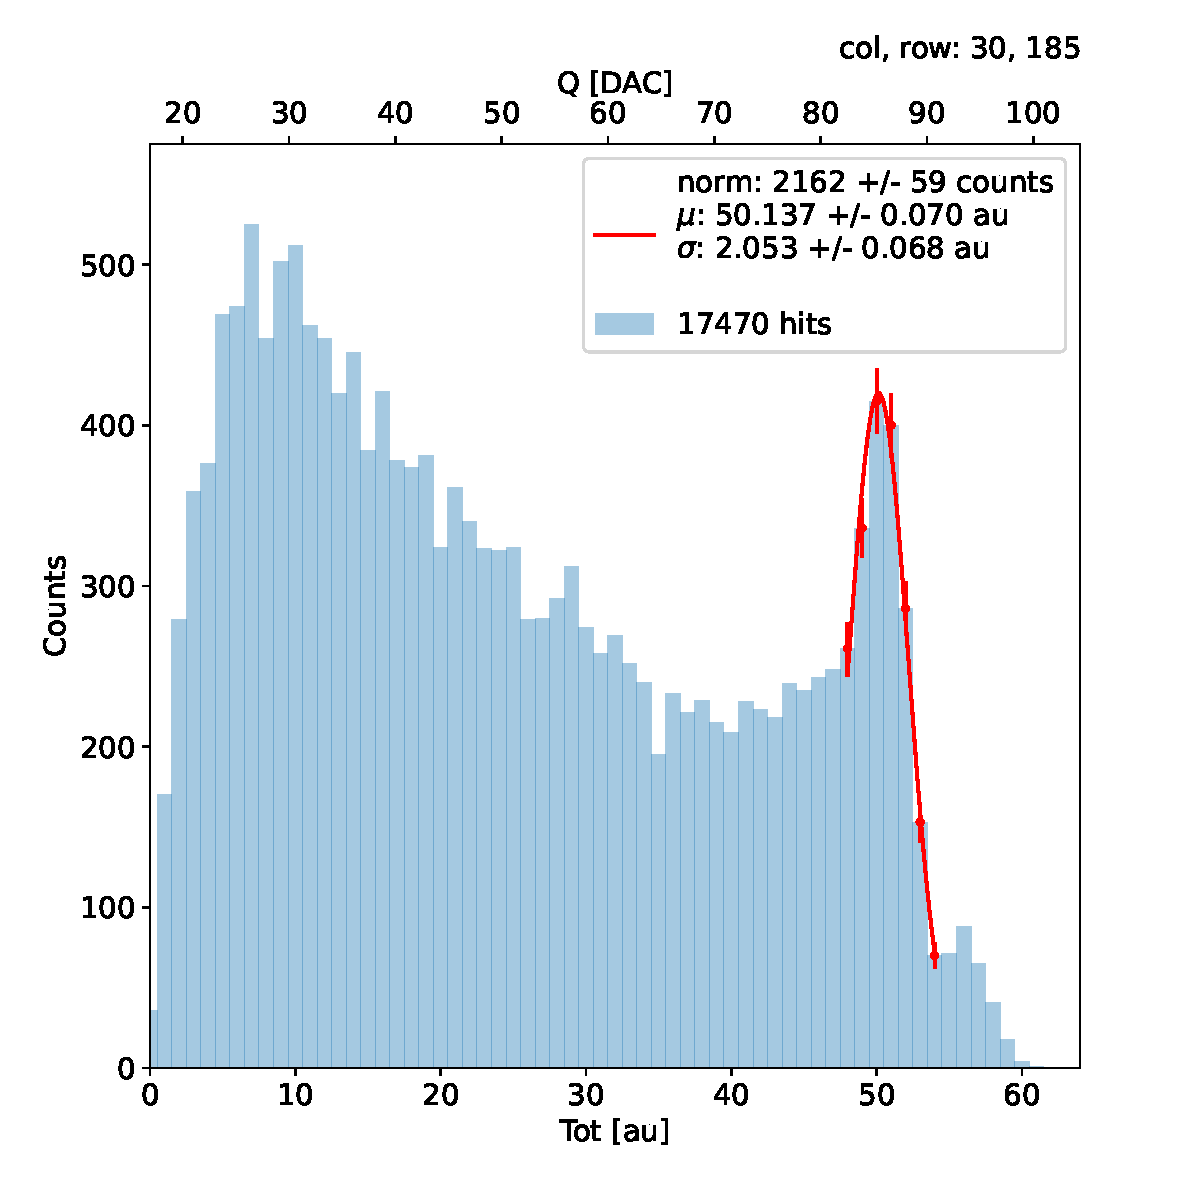
\includegraphics[width=.49\linewidth]{figures/charaterization/fit_gauss_r185.pdf}
            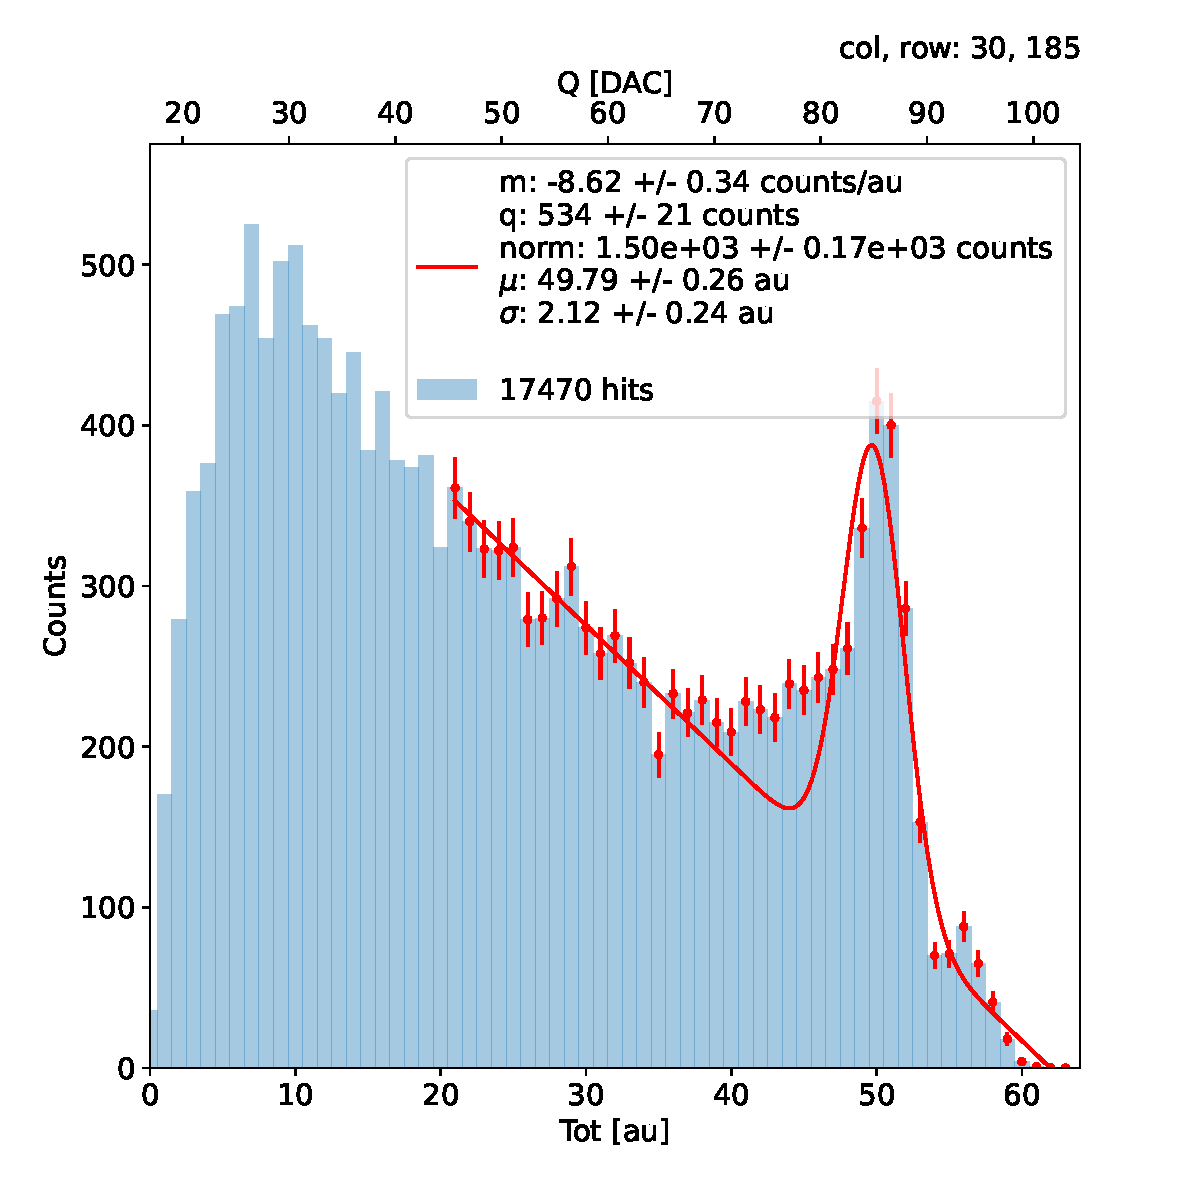
\includegraphics[width=.49\linewidth]{figures/charaterization/fit_line_gauss_r185.pdf}
            \caption{due pixel per far vedere la differenza tra i fit. Sottolinea che in rosso ci sono i bin fittati. La doppia scala utilizza le info trovate nel paragrafo precedente per il dato pixel in questione. Per avere una corrispondenza grezza in elettroni basta moltiplicare per 20 e- dac. }
        \end{figure}  
        %python3 -i acquisition_Fe55/fit_tot_single_pixel.py -f acquisition_Fe55/source_PMOSS/Fe_acquisitions_6V/ per fare i fit. Attenzione che prende i file degli istogrammi npz già
        Considering that the charge injected in the FE goes to fill capacitor which is different from pixel to pixel, the true charge injected does not correspond to what expected assuming C equal to \SI{230}{aF}, the nominal value. 
        Accordingly to that, a verification of the value provided and an absolute calibration of this capacity and of the conversion factor F is needed to have a correspondence of the signal in electrons; assuming C \SI{230}{aF}, F is expected to be \SI{20}{e-/DAC}, and is defined as:
        \begin{equation}
            F\, [e-/DAC] = \frac{1616\,e-}{Q\,[DAC]}
        \end{equation}

        For this pourpose a Fe55 radioactive source has been employed; the Fe55 is en extremely important radionuclide in the calibration of X-ray spectrometers, proportional counter and scintillator detector since it emits two two X-photons during the electron capture decay: the first one (K$_\alpha$) at \SI{5.9}{keV} and the second one (K$_\beta$) at \SI{6.5}{keV}.
        The K$_\alpha$ photon, which does photoelectric effect in the silicum, has an absorption length $\lambda$=\SIrange{7}{8}{\um}, and the probability of being assorbed in the \SI{25}{\um} thick epitaxyal layer is $\sim$0.95\.
        The electron emitted has an energy equal to the photon one, so recalling that the mean energy needed to produce a couple electron-vacuum is \SI{3.65}{eV}, the signal produced by the Fe55 source is expected to be \SI{1616}{e-}.
        In figures \ref{fig:fit_r185} and \ref{fig:fit_r69} are shown two histograms of the ToT spectrum of the Fe55 source for two different pixels. The peak corresponds to the events with completely absorption of the charge produced in the depleted region, while the long tail on the left to all the events with partial absorption due to charge sharing among neighbors pixels. In order to reduce the charge sharing, the pixel dimension in TJ-Monopix2 has been reduced down to 30$\times$\SI{30}{\um\squared}. 
        The events on the right side of the peak, instead, corresponds to the K$_{\beta}$ photons. 
        Looking at the histograms for pixel (30, 185) and (30,69) a significant difference in the peak to tail ratio leaps out. 
        This difference in the efficiency of detecting the signal can be related with the position of the pixel in the matrix: in particular pixels in the upper part of the matrix (rows 112-224) have a more prominent peak, while in pixels in the lower part (rows 0-111) there is a higher partial absorption. 
        I recall now that there is a slighly difference in the structure of the low dose-epi layer (\ref{chap:}) among the rows in the matrix, in particular pixels in rows 112-224 are supposed to have a higher efficiency in the pixel corner. 
        
        For the calibration I have need to establish the peak position; to do that I perform a fit of the ToT histogram of each pixels. As fit functions I test both the solutions below:  
        \begin{equation}
            f(x, N, \mu, \sigma) = \frac{N}{\sigma \sqrt{2\pi}} e^{-\frac{1}{2}(\frac{(x-\mu)}{\sigma})^2}
            \label{eq:gauss}
        \end{equation} 

        \begin{equation}
            f(x, m, q, N, \mu, \sigma) = m\,x + q + \frac{N}{\sigma \sqrt{2\pi}} e^{-\frac{1}{2}(\frac{(x-\mu)}{\sigma})^2}
            \label{eq:gauss_line}
        \end{equation}          
        \begin{figure}[h!]
            \centering
            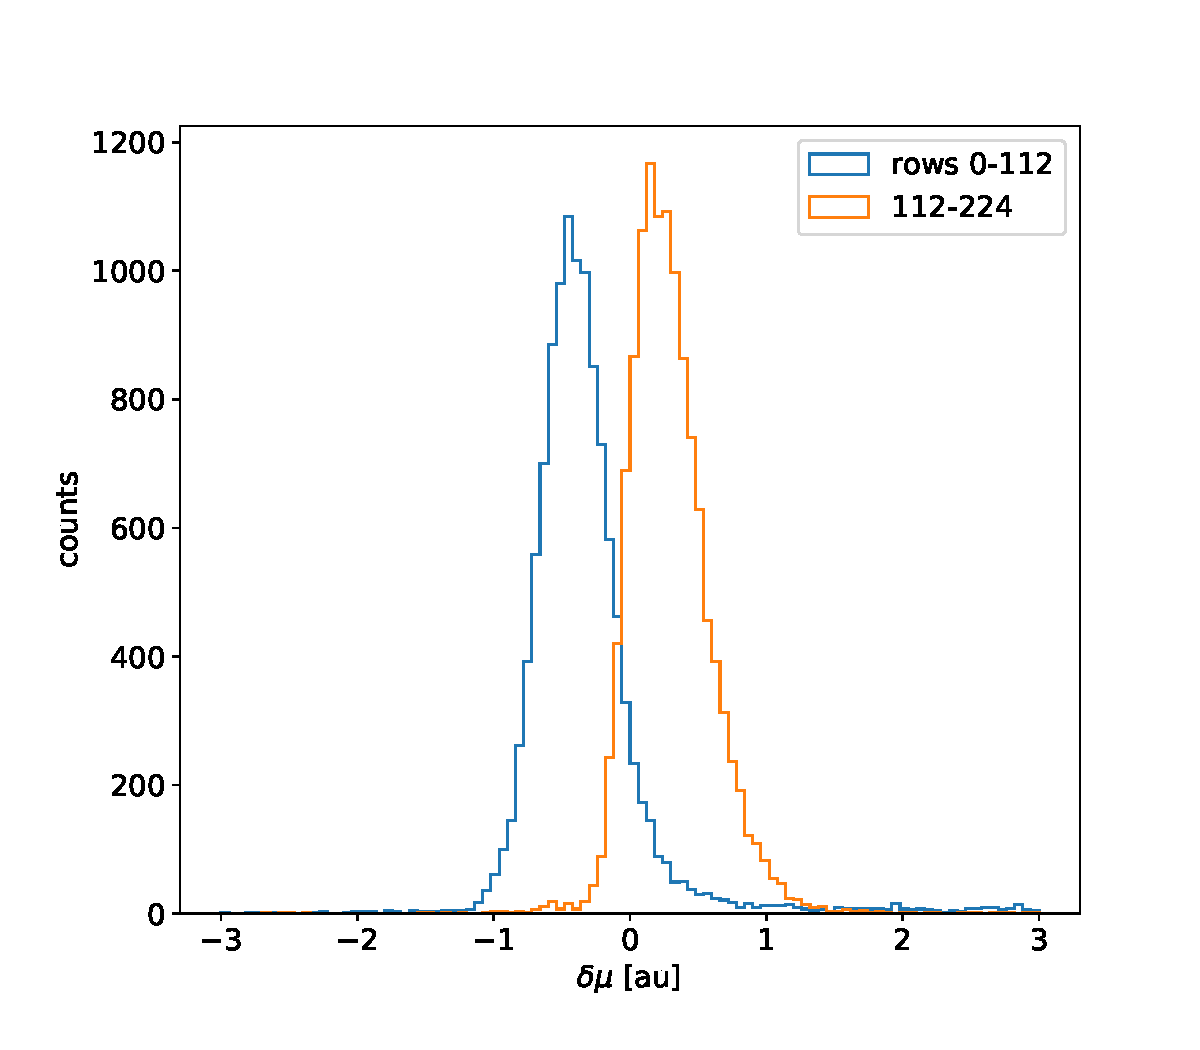
\includegraphics[width=.49\linewidth]{figures/charaterization/deltam_Fe.pdf}
            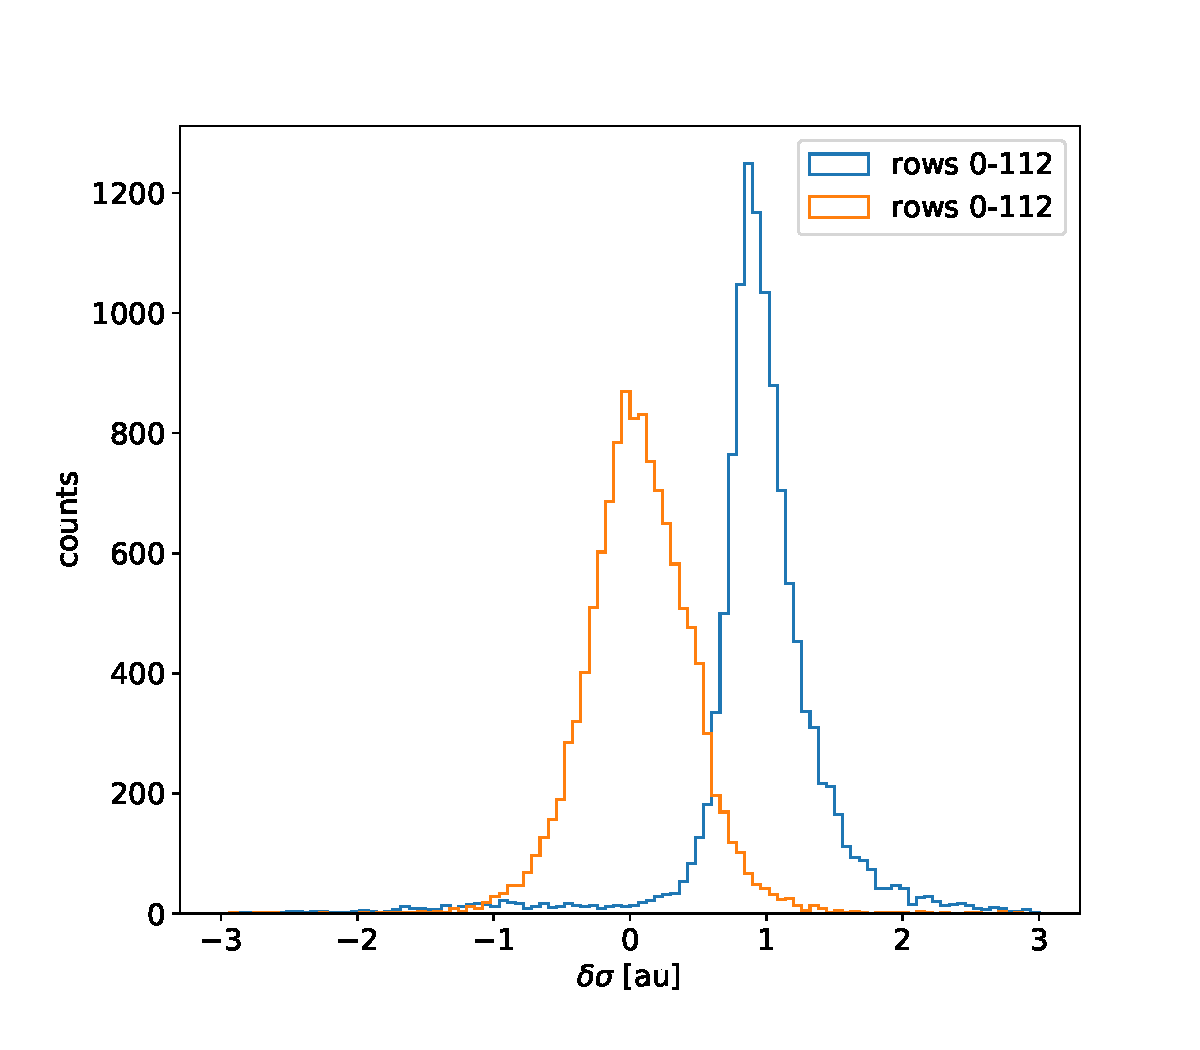
\includegraphics[width=.49\linewidth]{figures/charaterization/deltas_Fe.pdf}
            \caption{Here there are shown the defference between the parameters $\mu$ and $\sigma$ fitted with only a gaussian and with a gaussia plus a line. When $\mu<$0 the fit function \ref{eq:gauss} has given a worst peak (shifted on the left); when $\sigma<0$, \ref{eq:gauss_line} has given a worst peak width (larger sigma)}
            \label{fig:delta_fit}
        \end{figure}           
        \red{Nel primo caso ho fittato pochi pixel attorno a picco: il range è stato determinato .. controlla. 
        Nel secondo caso invece il range è..  Controlla sullo script  }  
        Even if the difference in the peak position between the two cases is not really relevant (\ref{fig:delta_fit}) being of the order of 0.8-1.5 \%,  it still introduces a systematic effect moving the peak on the left beacuse of the contribution of the tail. 
        Indeed, we know that the sharp edge on the right corresponds to the complete absorption of the photon, so excluding the little bump on the right, the more the fitted parameter is on the right, the better the fit is. Moreover, there is also systematic effect on the peak width, infact the worst fit also gives an overestimation of the peak width.  
        Even looking at the $\chi^2$, the fit function \ref{eq:gauss} seems so be the better choise, except for a sample of pixels on the lower part of the matrix, the one with lower efficiency.

        \red{Mappa del ferro da cui, come descritto enll'equazione si ricava la capacity.        
        La struttura a bande della capacità ha origine nel plot... e quindi nella calibrazione. 
        Andando a vedere gli istogrammi di queste due variabili si vedono dei picchi. C'è qualche struttura nella matrice che condiziona il funzionamento delle righe?
        Larghezza della gaussiana: fai il discorso a cosa contribuisce ad un picco così largo. è compatibile con quanto ti aspetti?}
        The voltage fluctuation around the peak is caused by the number fluctuation of generated carriers (Fano noise) and the noise introduced by the detector (sensor and front-end pre-amplifier).The ENC can be estimated from the standard deviation of the Kalpha voltage distribution. ENC = sqrt(sigma misurata- quella che ti aspetti dal fattore di Fano). E compatibile con quanto trovato? \red{se non fosse compatibile rimaneggia questa frase:tra noise is added from the system (test setup) at the analog monitoring pixel output.}
        \begin{figure}[h!]
            \centering
            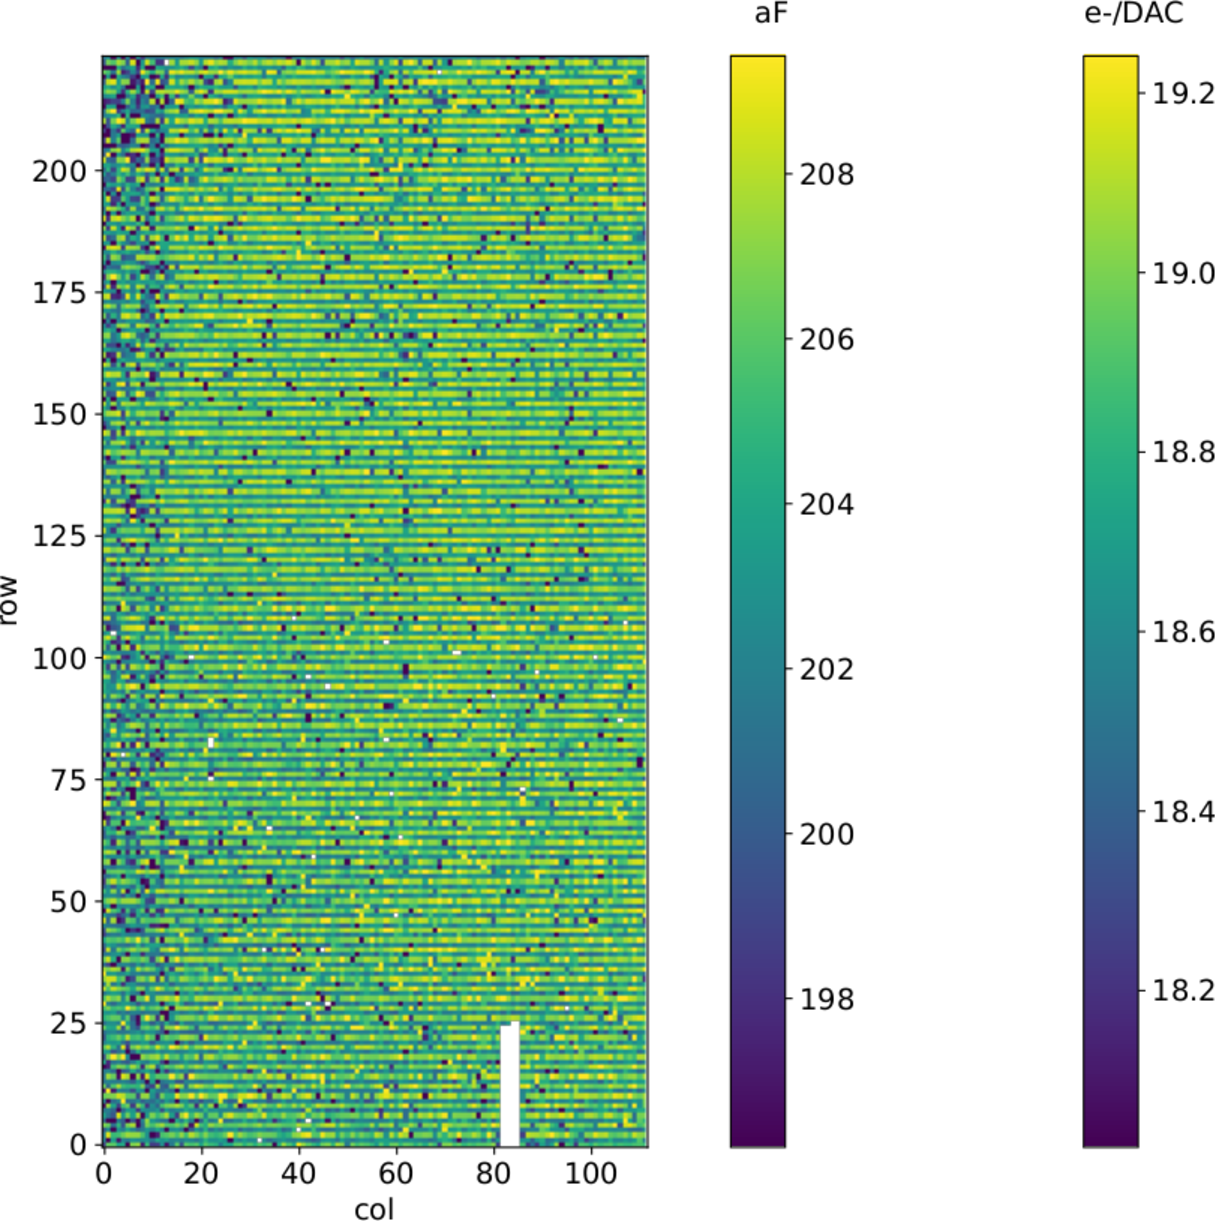
\includegraphics[width=.49\linewidth]{figures/charaterization/conversion_factor_map.pdf}
            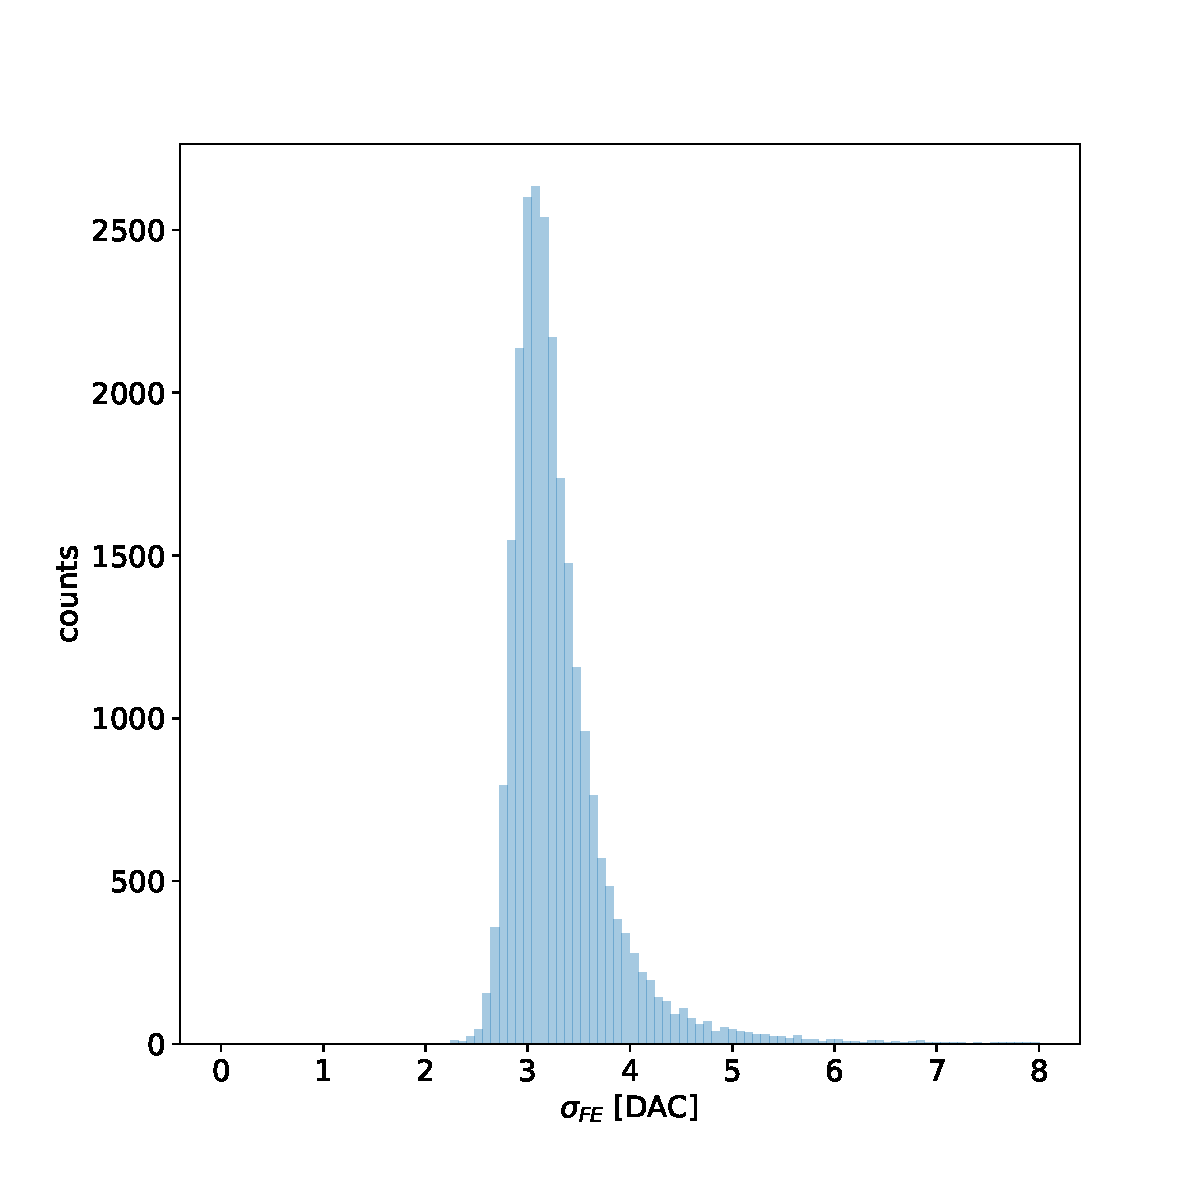
\includegraphics[width=.49\linewidth]{figures/charaterization/Fe_width_DAC_hist.pdf}            
            \label{fig:}
            \caption{}
        \end{figure}         


    \subsection{Changing the bias}\label{chap:characterization_section:bias}
        In order to study the behavior of the sensor changing the bias, I perform some injection scans in different configurations. 
        The thickness of the depletion has to be considered indeed an important parameters for the efficiency of the signal, and in particular it affects the charge released by a particle which cross the sensor (since the signal is proportional to the thickness of the epitaxial layer).
        Given that the chip under examination has a gap in the low dose epi-layer (look at chapter \ref{chapter:TJMonopix1_thesensor}) we were not able to change independently the bias of the substrate (PSUB) and of the p-well (PWELL), but they must be kept at the same value, differently from other chips, where on which some test has been performed, as reported in figure \ref{fig:gain_vs_bias}.
        A 2D map of the measured output voltage amplitude and resulting gain in the case of the PMOS and HV are reported. 
        \begin{figure}[h!]
            \centering
            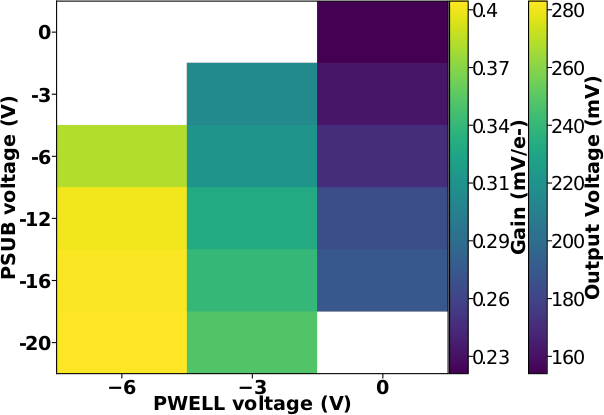
\includegraphics[width=.45\linewidth]{figures/Monopix1/PMOS_gain_bias.png}
            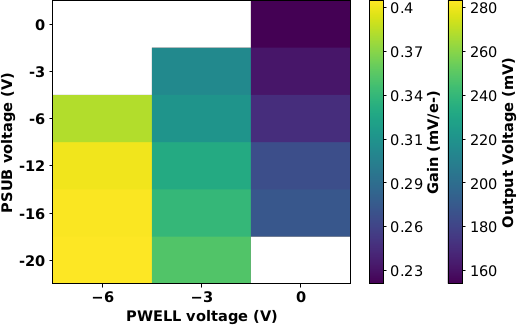
\includegraphics[width=.49\linewidth]{figures/Monopix1/HV_gain_bias.png}            
            \caption{2D map of the output voltage amplitude and gain with respect to the p-well and p-substrate in the case of the PMOS reset front-end (B)}
            \label{fig:gain_vs_bias}
        \end{figure}  

        In order to test the behavior of the chip when not completely depleted, I have performed an injection scan with PSUB/PWELL bias at \SI{0}{V}, -\SI{3}{V} and -\SI{6}{V}, and some acquisitions with the Fe55 source.
        The results of the measurements are reported in table \ref{tab:parameters_vs_bias} and in figure \ref{fig:Fe_spectrum_bias}.
        Turning down the bias, the depletion region narrows and the efficiency reduces, in particular in the pixel corner; in particular the threshold increases of $\sim$1/4, the noise of $\sim$1/3 and the slope, which parameterizes the linearity of the analog output and strictly depends on the gain, decreases of $\sim$1/4.
        In figure \ref{fig:Fe_param_vs_bias}(b) are reported the values of the K$_\alpha$ peak position, the normalization of the events above the peak and the rate, everything has been normalized to the value at the reference condition, which is with PSUB/PWELL at -\SI{6}{V}. 
        In order to evaluete the peak position and the normalization I have fit the spectrum in the region on the right with a gaussian.
        Looking at the spectrum, an other characteristics seems to appear: at lower bias the peak width is bigger than in a full depletion mode.
        This could be due at a bigger capacity, which influence the noise.         
    \begin{table}
            \begin{center}
            \begin{tabular}{| c |  c | c | c |}
            \hline
               & -\SI{6}{V} & -\SI{3}{V} & \SI{0}{V}\\
            \hline
            \hline
            Threshold [DAC] & 20.04 $\pm$ 1.6 & 21.0 $\pm$ 1.6 & 24.5 $\pm$ 1.8\\
            Noise [DAC] & 0.613 $\pm$ 0.075 & 0.625 $\pm$ 0.078 & 0.822 $\pm$ 0.098\\
            Slope [au/DAC] & 0.726 $\pm$ 0.027 & 0.707 $\pm$ 0.028  & 0.573 $\pm$ 0.021\\
            Offset [au] & -10.8 $\pm$ 1.9 & -11.2 $\pm$ 1.8 & -11.1 $\pm$ 1.5 \\
            \hline
            \end{tabular}
            \caption{The errors are the standard deviations of the corresponding distributions. The conversion factor from DAC to electrons is $\sim$\SI{20}{e-/DAC}.}
            \label{tab:parameters_vs_bias}
            \end{center}
        \end{table}  
        
        \begin{figure}[h!]
            \centering
            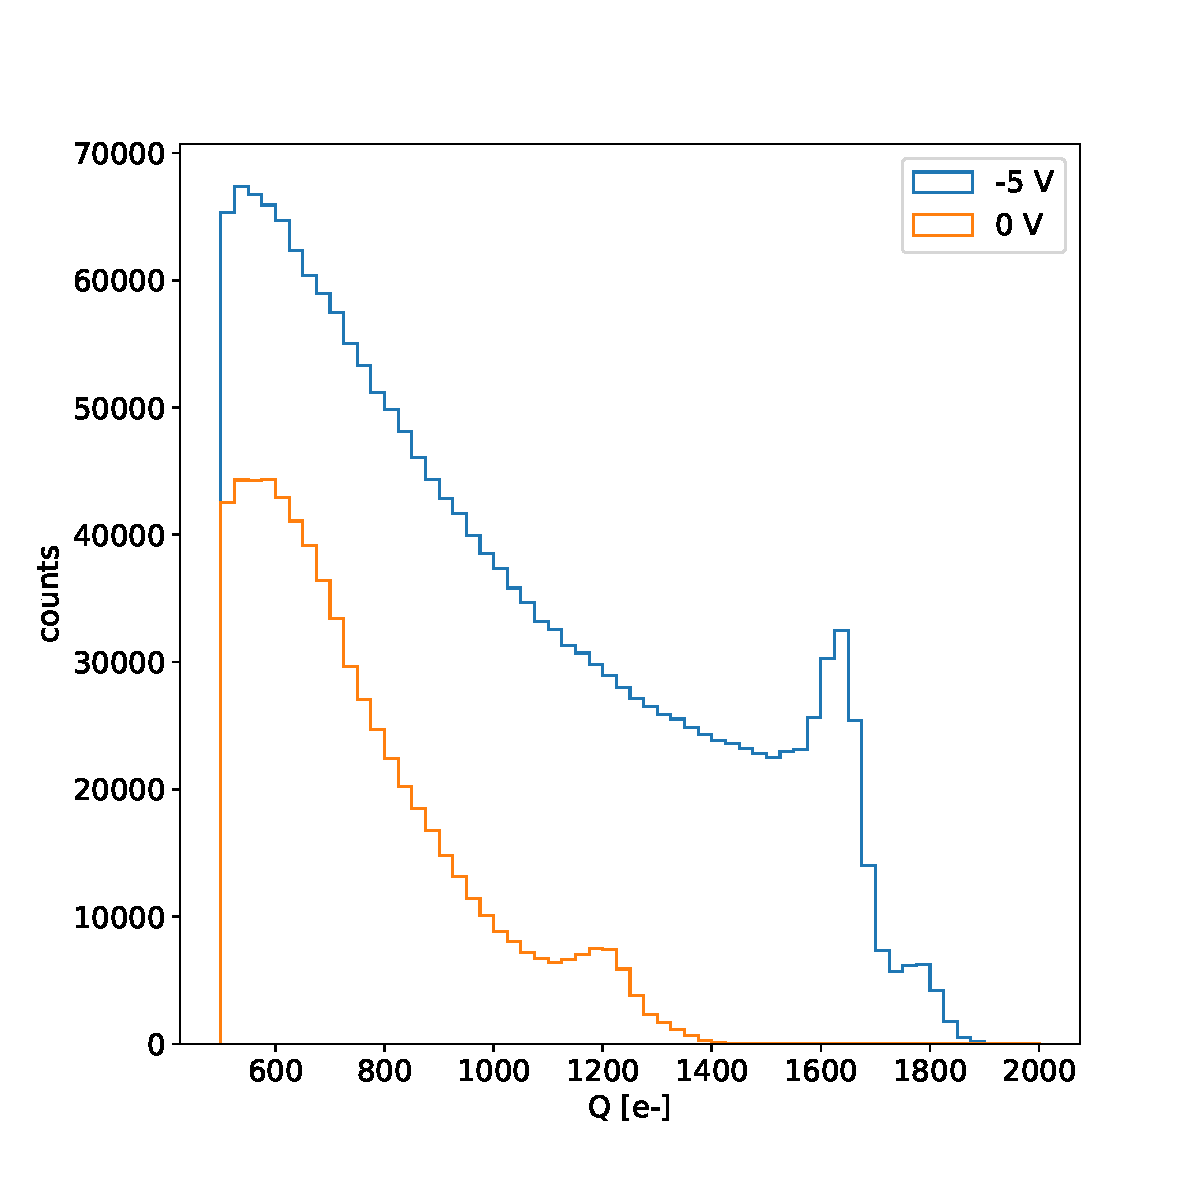
\includegraphics[width=.60\linewidth]{figures/charaterization/Fe_spectrum_bias.pdf}
            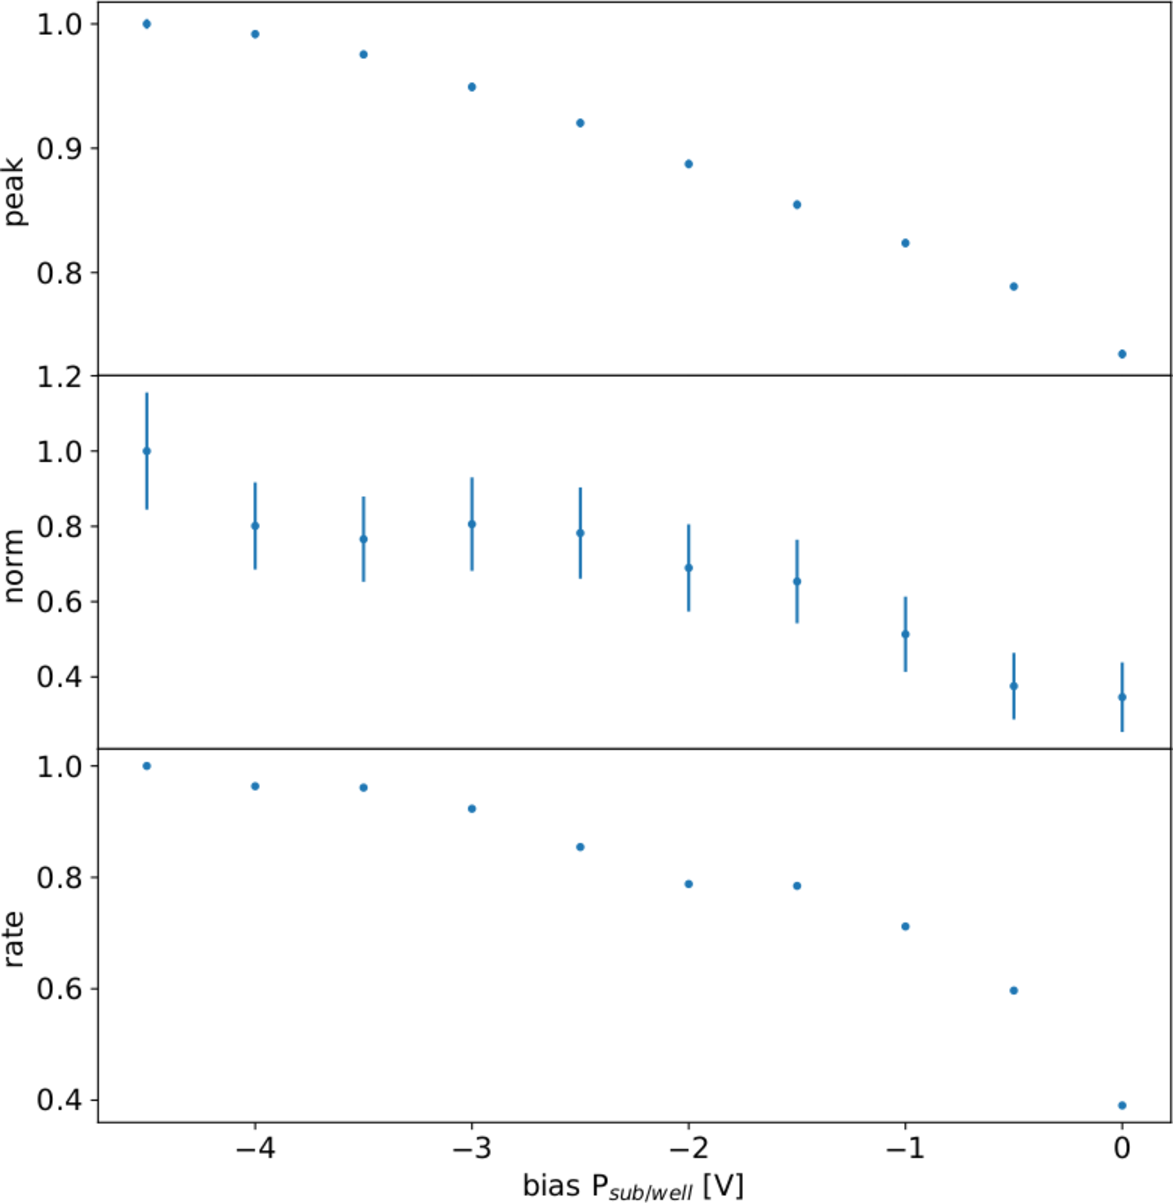
\includegraphics[width=.70\linewidth]{figures/charaterization/Fe_param_vs_bias.pdf}
            \caption{Two acquisition with the Fe55 source at different bias. }
            \label{fig:Fe_param_vs_bias}
        \end{figure}     


    \subsection{Measurements with radioactive sources}
        %python3 -i acquisition_Fe55/find_cluster.py -d acquisition_Fe55/source_PMOSS/noise_acquisitions_6V -> per cluster dimension e spettro del noise
        %python3 -i acquisition_Fe55/hit_map.py -f acquisition_Fe55/source_PMOSS/2022-04-07/2022-04-07_10-10-01_acq.h5 -> per le hit map, comprese qualche hitmap dei cluster
        %python3 -i acquisition_Fe55/Sr90_spectrum.py -d acquisition_Fe55/source_PMOSS/noise_acquisitions_6V/ -> per fare i plot dello stronzio
        In order to completely validate the operation of the whole sensor\footnote{As I will explained in chapter \ref{chap:} these measurements are foundamental also to be compared with the spectrum seen at the testbeam}, I have made some acquisitions with radioactive source, in particular I have used Fe55, Sr90, which is a $\beta^-$ emettitor with electron endpoint at \SI{0.546}{MeV}, and cosmic rays, which are supposed to be mostly MIP. 
        In the acquisitions with Sr90 and cosmic rays, I specifically focused on the events whith charge sharing and with more hits than one per events, that are clusters.

        The definition of cluster I chose is built only on the time of arrival of hit, in particular I established that all particles with the same timestamp belong to the same cluster.
        This obviously is a coarse requirement but it gave me the opportunity of using a simple and fast clustering algorithm, which is fine when the random coincidence probability is neglibile. 
        Defining R$_1$ and R$_2$ as the two events rate, and $\tau$ as the dead time of the detector, the random coincidence rate can be found: 
        \begin{equation}
            R_{coinc} = R_1 \, \times\, R_2 \, \times \, \tau
        \end{equation}
        As I am going to prove in the next section, the dead time strictly depends on the occupancy of the matrix, even through we can assume a dead time of $\sim$\SI{1}{\um}, which corresponds to the mean dead time per pixel. However, if in an event a particle hit two different pixels producing a cluster, the total dead time simply doubles.   
        Then, assuming a rate of noise of $\sim$\si{Hz} on the whole matrix and being the mean rate of the , the random coincidence of two hits coming from Fe-noise, Sr-noise, CR-noise and noise-noise are respectively 
        
        In figure \ref{fig:cluster_dimensions} I report the histograms of the number of pixels in the cluster and of the dimension of clusters, defined in terms of the max and min coordinates on the matrix as:
        \begin{equation}
            d = \sqrt{(y_{max}-y_{min})^2 + (x_{max}-x_{min})^2}
        \end{equation}
        \red{quello che si nota è che lo Sr  fa cluster più grandi mediamente, che arrivano anche a 22 hit.}

        Below I have also attached a sample of hitmap of events produced by the three different sources. 


        \begin{figure}[h!]
            \centering
            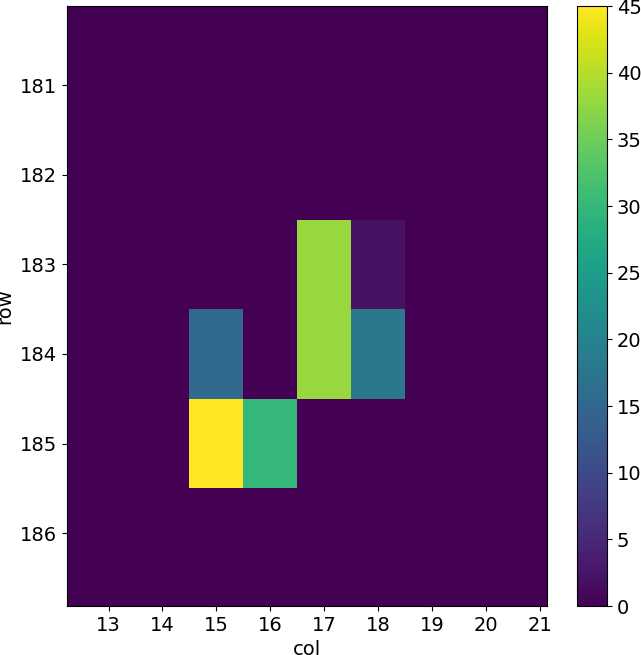
\includegraphics[width=.24\linewidth]{figures/charaterization/evts/cosmic_rays/7a.png}
            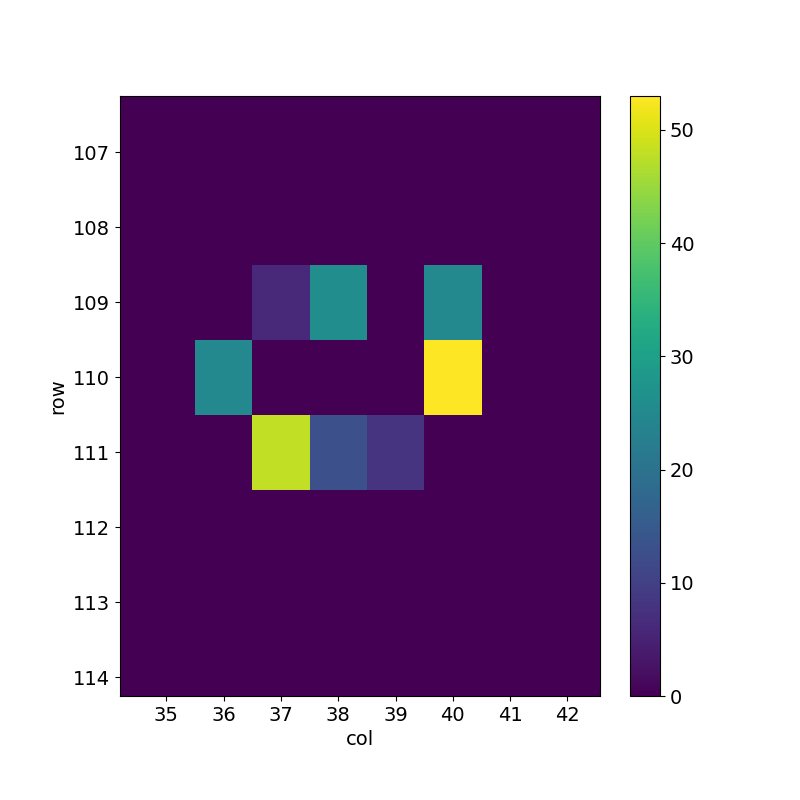
\includegraphics[width=.24\linewidth]{figures/charaterization/evts/cosmic_rays/8a.png}
            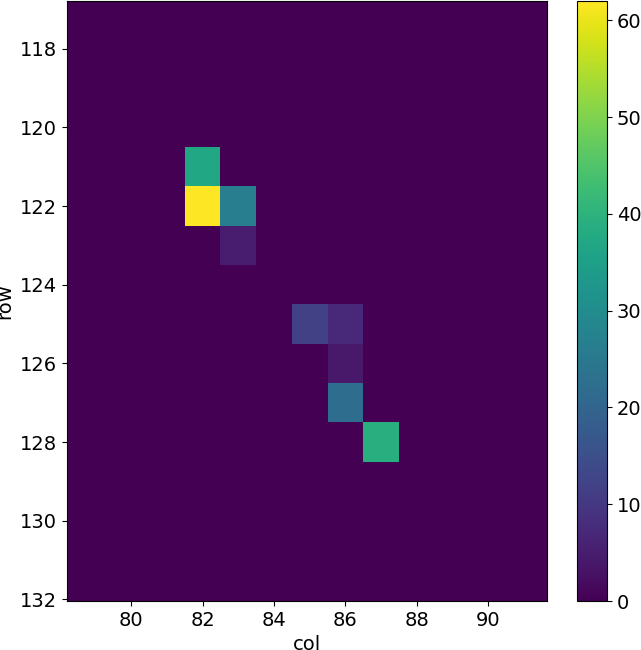
\includegraphics[width=.24\linewidth]{figures/charaterization/evts/cosmic_rays/9c.png}\\       
            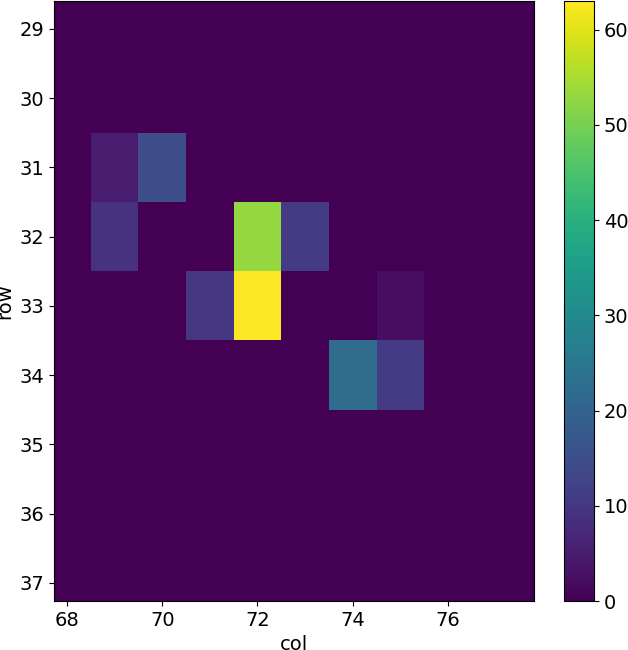
\includegraphics[width=.24\linewidth]{figures/charaterization/evts/cosmic_rays/10a.png}
            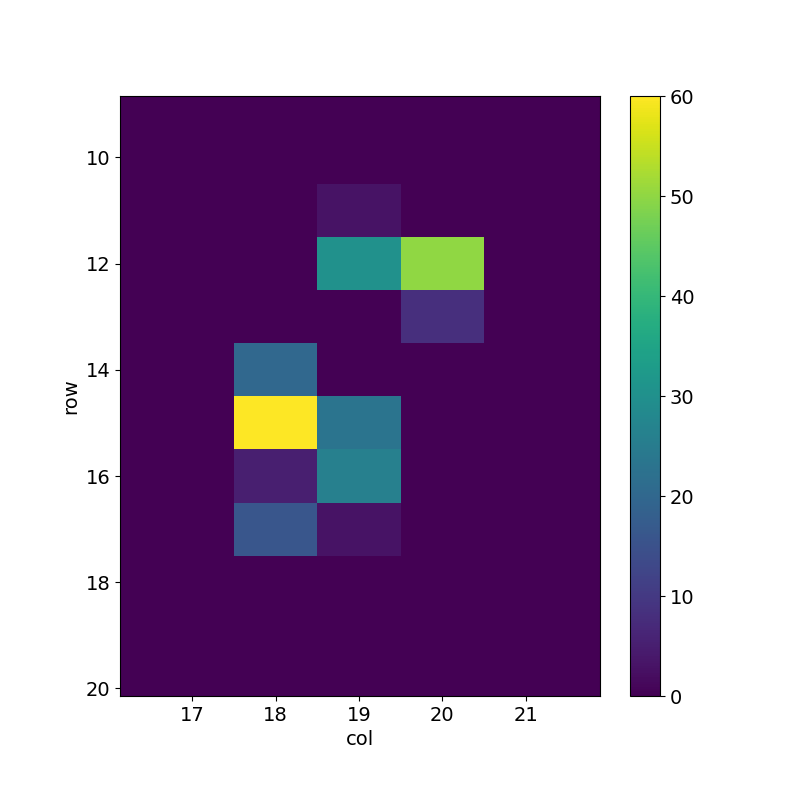
\includegraphics[width=.24\linewidth]{figures/charaterization/evts/cosmic_rays/11a.png}
            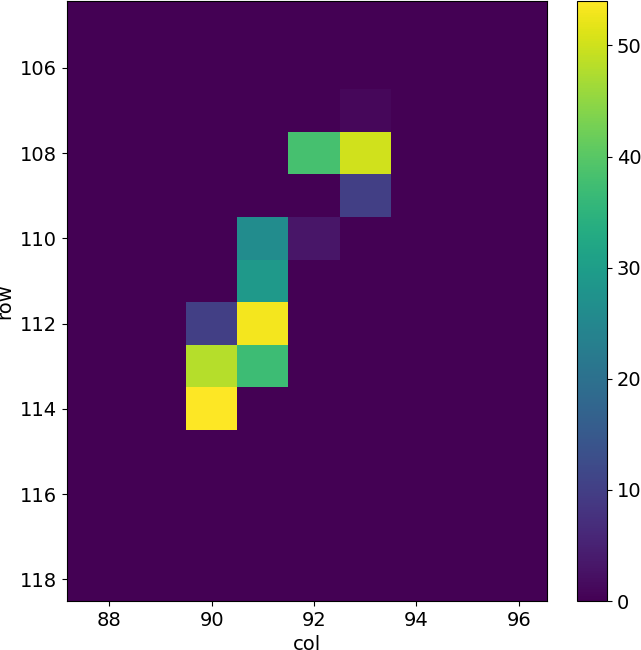
\includegraphics[width=.24\linewidth]{figures/charaterization/evts/cosmic_rays/12.png}
            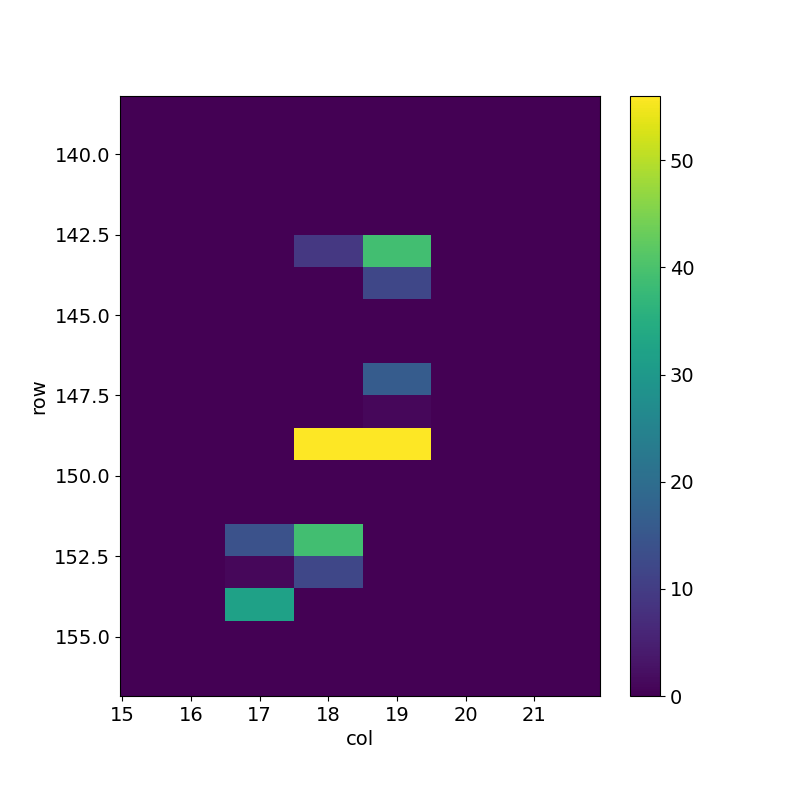
\includegraphics[width=.24\linewidth]{figures/charaterization/evts/cosmic_rays/12b.png}               
            \caption{ }
            \label{fig:hit_map_cosmic_rays}
        \end{figure} 


        \begin{figure}[h!]
            \centering
            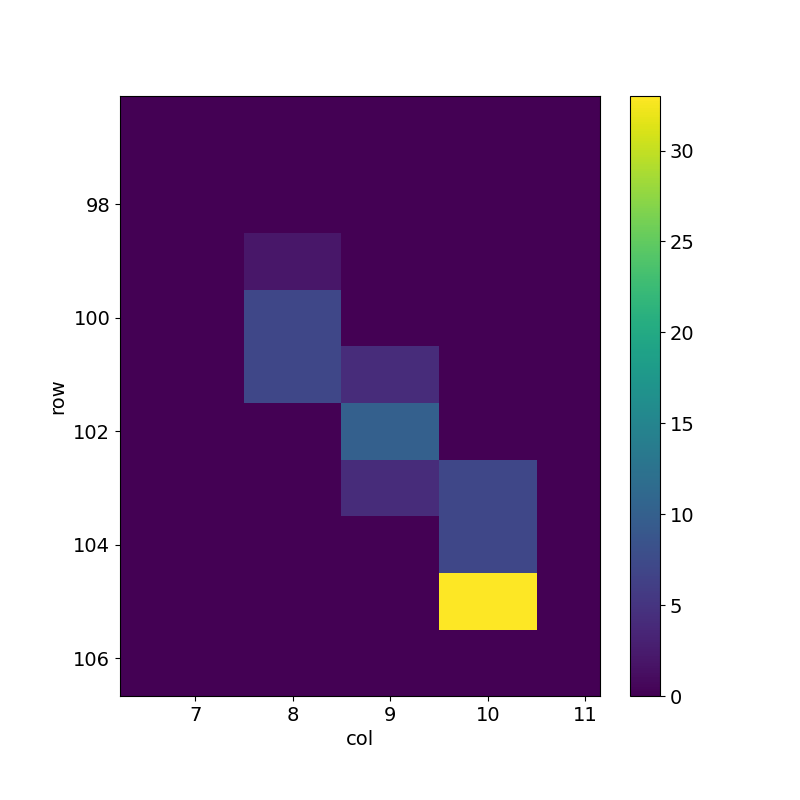
\includegraphics[width=.24\linewidth]{figures/charaterization/evts/Sr90/9b.png}
            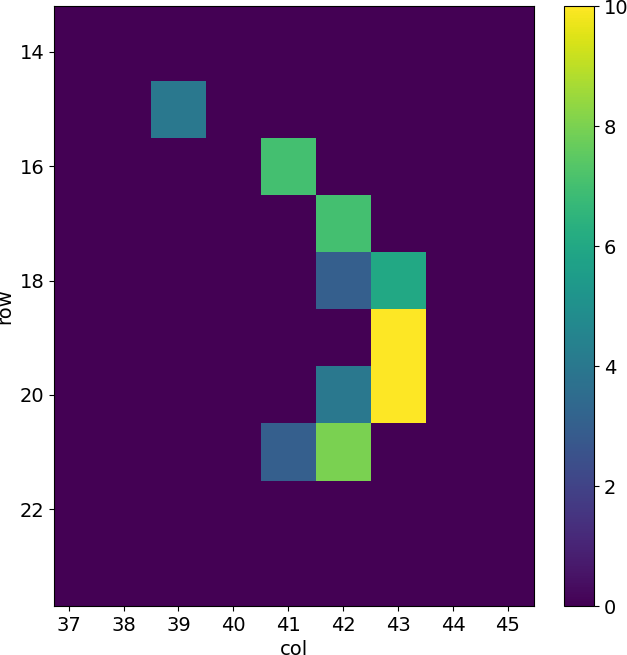
\includegraphics[width=.24\linewidth]{figures/charaterization/evts/Sr90/10b.png}
            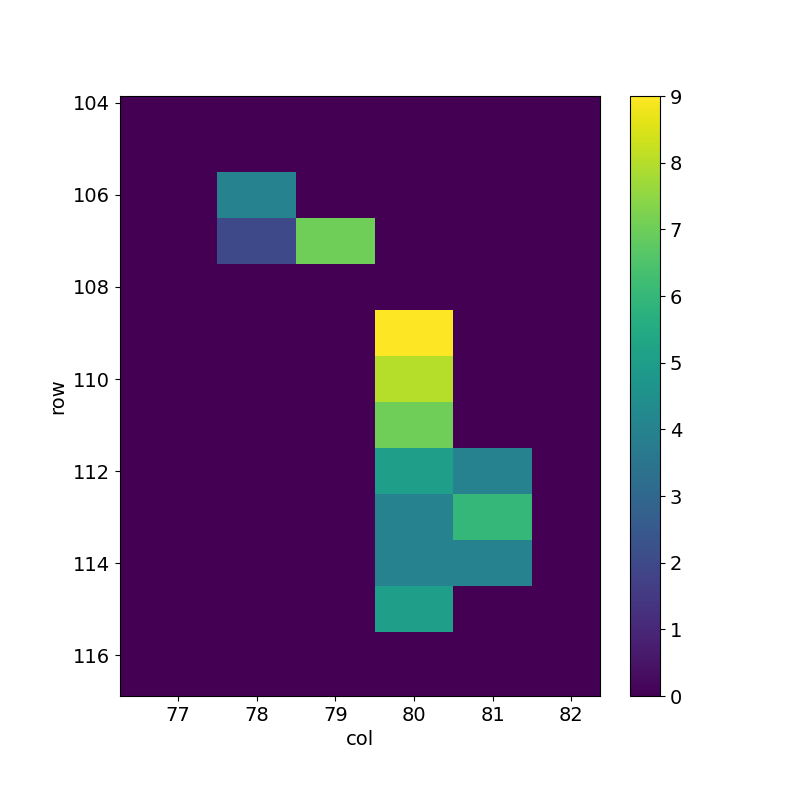
\includegraphics[width=.24\linewidth]{figures/charaterization/evts/Sr90/13a.png}
            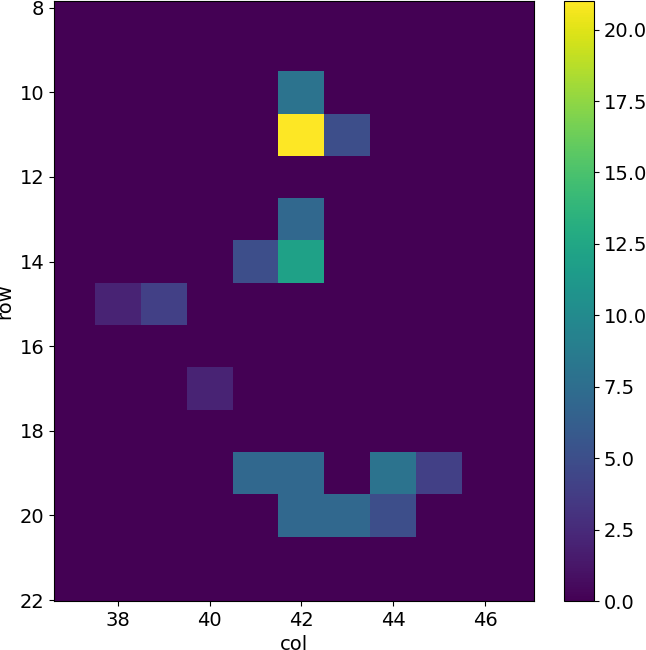
\includegraphics[width=.24\linewidth]{figures/charaterization/evts/Sr90/16a.png}\\
            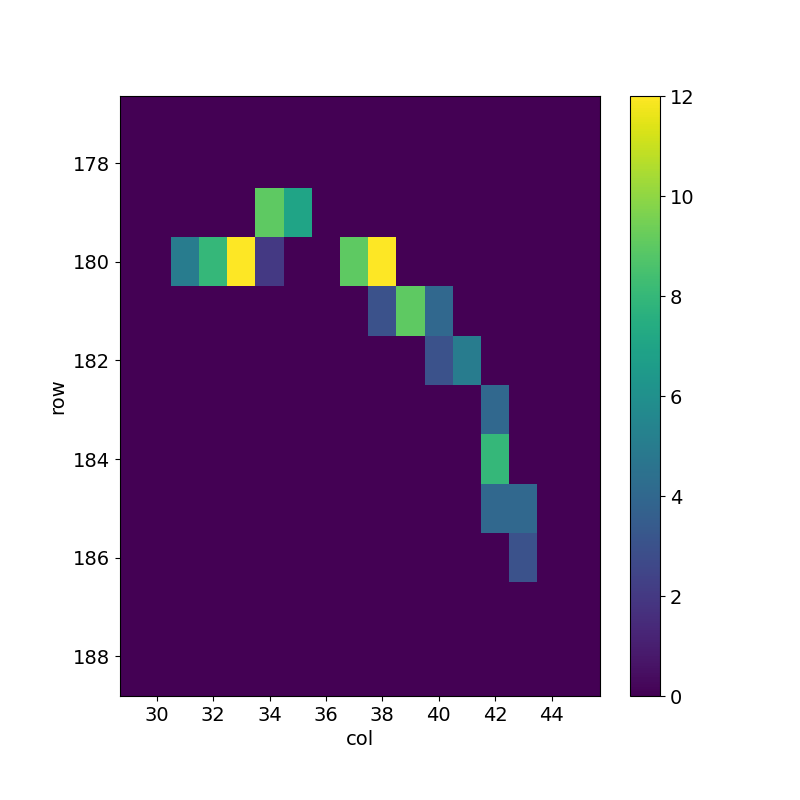
\includegraphics[width=.24\linewidth]{figures/charaterization/evts/Sr90/18b.png}
            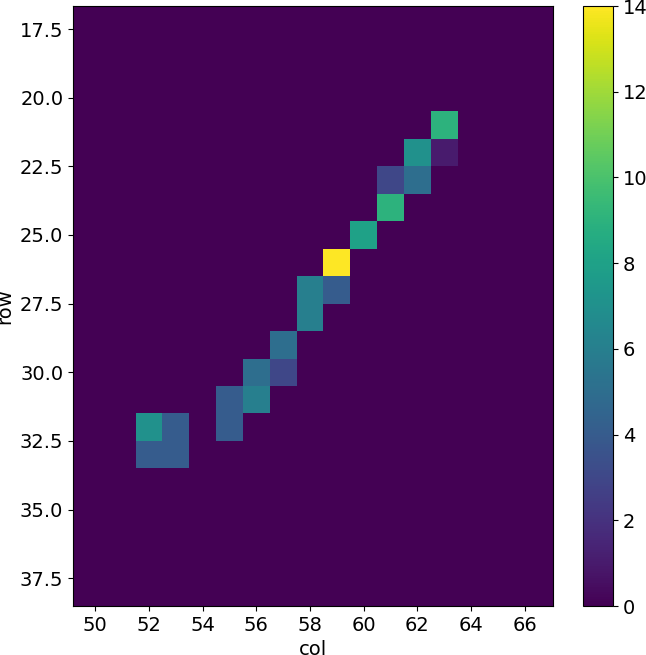
\includegraphics[width=.24\linewidth]{figures/charaterization/evts/Sr90/21a.png}
            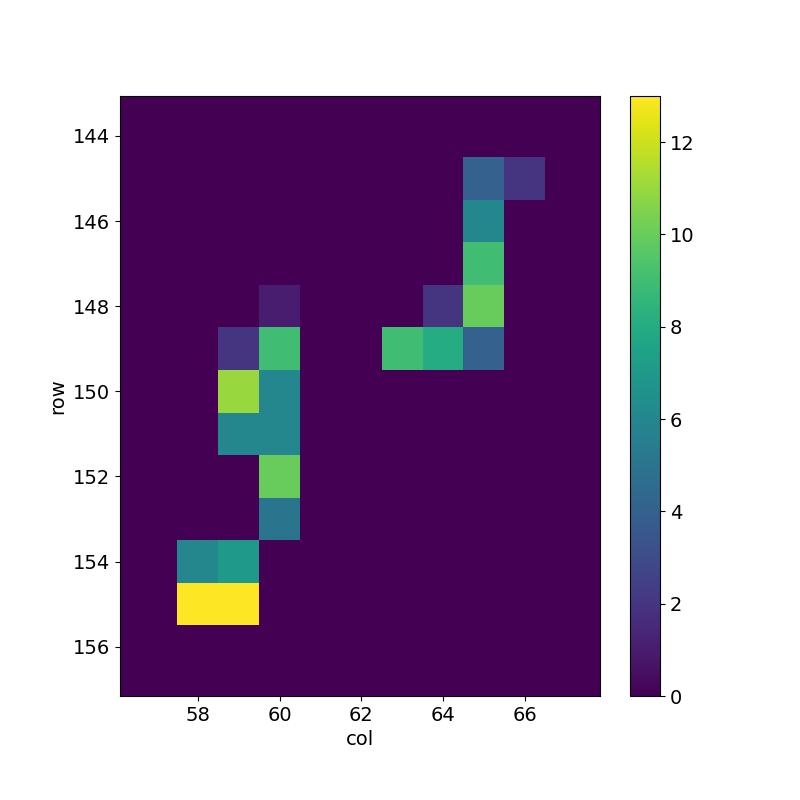
\includegraphics[width=.24\linewidth]{figures/charaterization/evts/Sr90/22a.png}
            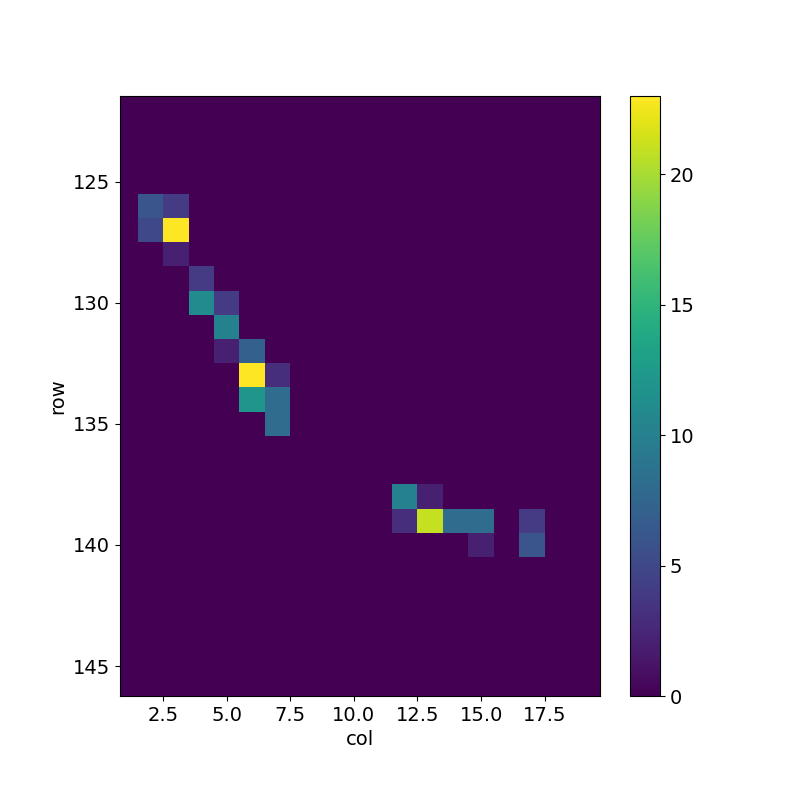
\includegraphics[width=.24\linewidth]{figures/charaterization/evts/Sr90/25a.png}               
            \caption{ }
            \label{fig:hit_map_Sr90}
        \end{figure}         

        \begin{itemize}
            \item PLOT delle hit per cluster
            \item  esempio di hitmap di cluster
            \item sostituisci in carica in un file del ferro, guarda somma dei cluster, stessa cosa per Sr e MIP
            \item  Spiega che con il flavor HV abbiamo una perdita di sengnale, fai vedere uno spettro di delle misure dell 8 marzo. 
        \end{itemize}
        The signal generated by electrons is similar to the one generated by minimum ionizing particle (MIPS) \red{dovrei mettere qualche conto per giustificare questa affermazione}, and the spectrum is expected to follow a Langau-Gauss distribution.
        \red{nelle acquisizioni dei CR ho selezionato solo i cluster, per tagliare via il rumore.}
        
        , looking at the cluster dimension and the cluster charge.  


    \subsection{Dead time measurements}
        The hit loss is due to analog and digital pile up: the first one occurs when a new hit arrives during the pre-amplifier response, the second instead when the hit arrives while the information of the previous hit has not yet been transferred to the periphery.  
        Since the pre-amplifier response has a characteristic time $\sim$ToT, the dead time $\tau_{a}$ introduced by it will be at most \SI{1.6}{\us}; using the IRESET and VRESET FE parameters the reset time can be lowered down, but a \red{IRESET, puoi diminuire il tempo di scarica.}   
        Regarding the latter contribution instead, since only one hit at a time can be stored on the pixel's RAM, until the data have completed the path to get out, the pixel is paralyzed. Moreover since there is no storage memory included on TJ-Monopix1 prototypes, the digital dead time $\tau_{d}$ almost corresponds to the time needed to trasmit the data-packets off-chip. 

        The exportation of data from pixel to the EoC occurs via a 21-bits data bus, therefore only one clock cycle is needed and the dead time bottleneck is rather given by the bandwidth of the serializer which trasmits data off-chip from the EoC. In our setup the serializer operates at 40 MHz, thus to transmit a data packet (27-bit considering the addition of 6 bits to identify the double-column at the EoC) at least \SI{675}{ns} are needed. 
        For what we have said so far, the R/O is completely sequential and therefore is expected a linear dependence of the reading time on the number of pixels to read:
        \begin{equation}
            \tau =\, 25\: \unit{ns}\, \times\, (\alpha\, N +\, \beta)
            \label{eq:reading_time}
        \end{equation}
        where $\alpha$ and $\beta$ are parameters dependent on the readout chain setting. 
        
        To test the linearity of the reading time with the number of pixels firing and to measure it, I have used the injection circuit which allows me choosing a specific hit rate: I made a scan injecting a fix number of pulses and each time changing the number of pixels injected.
        Indeed the injection mode allows fixing not only the amplitude of the pulse, which corresponds to the charge in DAC units, but also the time between to consecutive pulses (DELAY) and the width (WIDTH). The hit rate then corresponds to :
        \begin{equation}
            R = \frac{\SI{25}{ns}}{(DELAY+WIDTH)}
        \end{equation}
        where WIDTH is equal to \SI{60}{counts}. 

        Unfortunately a high random hit rate on the matrix cannot be simulated by the injection because of the long time ($\sim$\si{ms}) needed to set the pixel registers of the injection; then I was forced to specify at the start of the acquisition the pixels to inject on, and for convenience I chose those on a same column.  
        In figure \ref{fig:efficiency_VS_delay} is shown the dependence of the efficiency on the DELAY parameter in two different cases. 
        For the 5 pixels example the efficiency goes down the 90\% at a DELAY of $\sim$185 clock counts, which corresponds to \SI{6.125}{\us} and to a rate of \SI{160}{kHz}, while in the 10 pixels example, the efficiency goes under the 100\% at $\sim$\SI{380}{clock} counts, which corresponds to \SI{11}{\us} and to a rate of \SI{90}{kHz}. 
        \red{COME MAI SONO DIVERSE LE CURVE?}
        \begin{figure}[h!]
            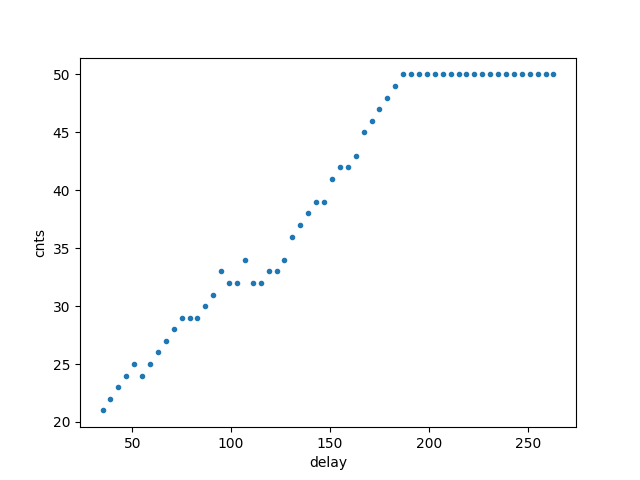
\includegraphics[width=.49\linewidth]{figures/charaterization/efficiency_5pixels.png}
            \centering
            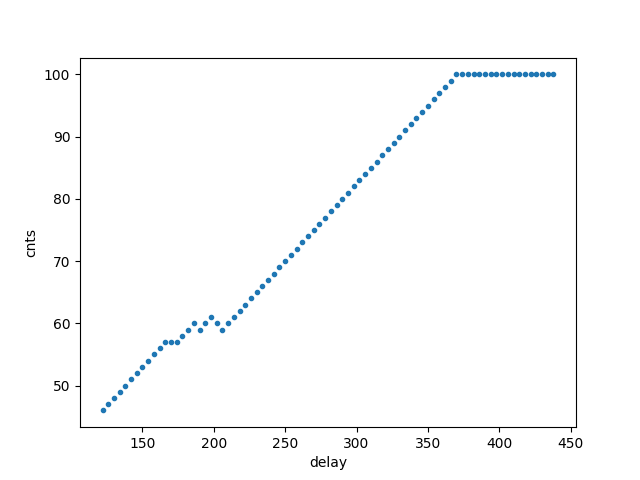
\includegraphics[width=.49\linewidth]{figures/charaterization/efficiency_10pixels.png}
            \caption{Efficiency vs the DELAY parameters. (a) I made a scan injecting 5 pixels with 50 pulses for each DELAY configuration and (b) 10 pixels with 100 pulses for each DELAY}
            \label{fig:efficiency_VS_delay}
        \end{figure}
        From the efficiency curves I have then looked for the time when the efficency decreases. In figure \ref{fig:dead_time}(a) is shown the dead time per pixels as a function of N with different R/O parameters configuration, the meaning of which is explained in chapter \ref{chap:Monopix_RO}. The default value suggested by the designer of the chip are reported in table \ref{tab:R/O_param}; moving too much the readout parameters from the default ones, the readout does not work properly, and no hits can be read at all. The problem probably stays in the firmware setting of the readout which are specially fixed for our chip \red{Sul repositorio, nei commenti ci sono altri valori possibili per il FREEZE, ma avevamo detto che probabilmente sono relativi ai setting di altri chip.}
        %Cambiando molto i parametri del R/O la lettura non funzionava per niente: ad esempio CONF\_STOP\_FREEZE non può essere impostato nè sopra 105 nè sotto 95
        Despite the single pixel reading time does not depend on the position on the pixel matrix, whithin a clock count which is $\sim$\SI{25}{ns}, and it is equal to \SI{106}{clock} counts, since the $\tau_d$ critically depends on the pixel position on the matrix: in particular the reading sequence goes from row 224 to row 0, and from column 0 to column 112, making the pixel on the bottom right corner the one with the longest dead time. 
       
        \begin{table}
            \begin{center}
            \begin{tabular}{|c | c | c |}
            \hline
            Parameter & Value [\si{DAC}] & Value [\si{\us}]\\
            \hline
            \hline
            START\_FREEZE & 64 & 1.6\\
            STOP\_FREEZE & 100 & 2.5\\
            START\_READ & 66 & 1.65\\
            STOP\_READ & 68 & 1.7\\
            \hline
            \end{tabular}
            \caption{Default configuation of the R/O parameters}
            \label{tab:R/O_param}
            \end{center}
        \end{table}
        \begin{figure}[h!]
            \centering
            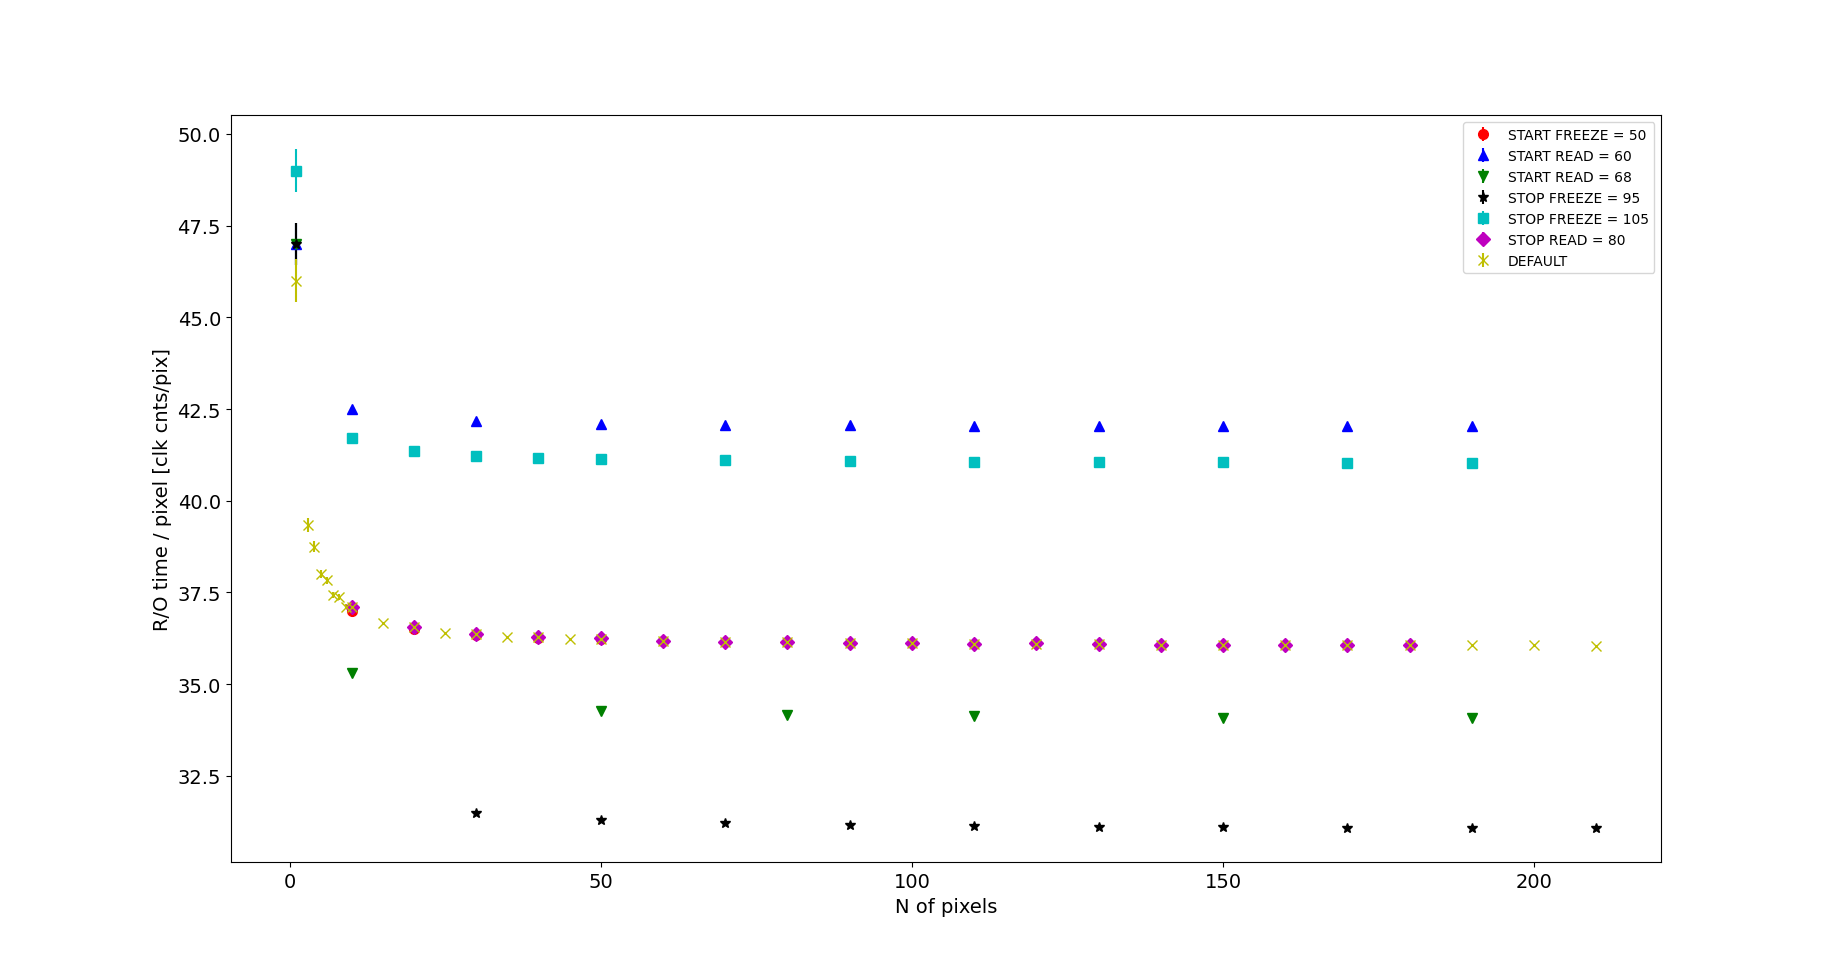
\includegraphics[width=.9\linewidth]{figures/charaterization/parameters_points.png}
            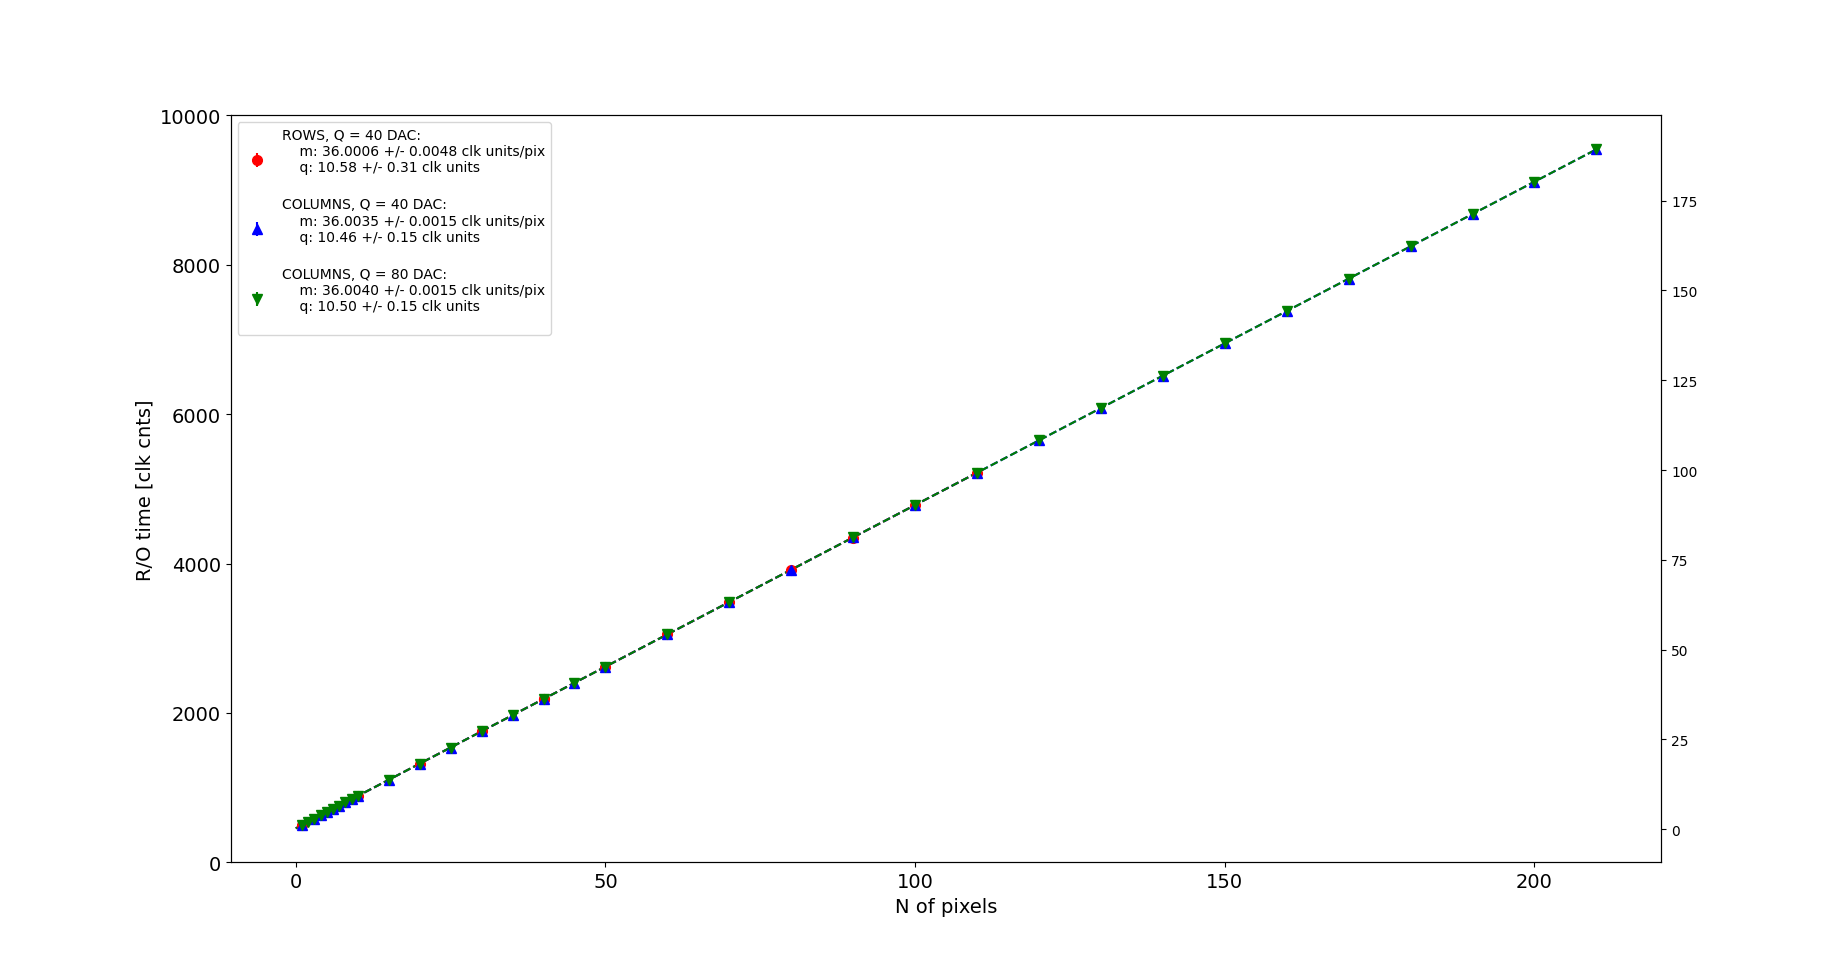
\includegraphics[width=.9\linewidth]{figures/charaterization/default_line.png}
            \caption{(a) Readout time per pixel as a function of the number of pixel injected obtained with different FE setup. (b) Readout time as a function of the number of pixels injected obtained injecting pulses with amplitude of \SI{80}{DAC} (green), of \SI{40}{DAC} on the same row (red) and on the same column (blue).}
            \label{fig:dead_time}
        \end{figure}
        Furthermore to test that there is no dependece of the digital readout time from the charge of the pulse, I have try to change the amplitude of the pulse injected, but the parameters found were consistent with the default configuration ones.
        No difference in the $\alpha$ and $\beta$ coefficients has been observed between the two case.
        \red{In realtà non mi torna perchè il FREEZE dovrebbe iniziare n cicli di clock dopo il TE, ed il TE dipende ovviamente dal ToT, quindi mi sarei aspetatta una differenza tra i due.}
        Referring to eq.\ref{eq:reading_time}, the factor $\alpha$ is proportional to the difference (STOP\_FREEZE - START\_READ), while the offset $\beta$ lies between 5 and 15 clock counts.

        Per avere una misura veritiera del tempo morto e del hit loss si dovrebbe iniettare casualmente input events are produced by a
        random hit generator with a specified hit rate, hence following a Poisson distribution. Inoltre faccio notare che il tempo morto è così lungo perchè c'è parallelizzazione e neppure un buffer (cosa tipicamente prevista quando li si inserisce nei rivaltori). Ad esempio Obelix, per l'upgrade di Belle2 avrà un buffer a fine matrice. 

\section{ARCADIA-MD1 characterization}
    Unfortunatly we have found out that the chip we received was not completely functional, then we have been able to make on it only a few electrical and software test. We have then verified the comunication of the chip with the DAQ, testing the operations of the FPGA and the breackout board (BB).  
    The problem occurs when the chip is biased, in particular, when the HV voltage is lowered down \SI{0}{V}, the sensor requires too much power and a too high current draw sets. We have discussed the problem with the designers of the chip whose helped us indentifying the motivation of the break: the chip has been glued using too much conductive tape and hence have a short-circuit between the sides and the back, which makes impossible the biasing.     
    Unfortunately, since both the sensor and the FE require at least -\SI{10}{V} to work properly, no measurement was possible except the acquisition of the noise in the FE circuit. 
    \begin{figure}[h!]
        \centering
        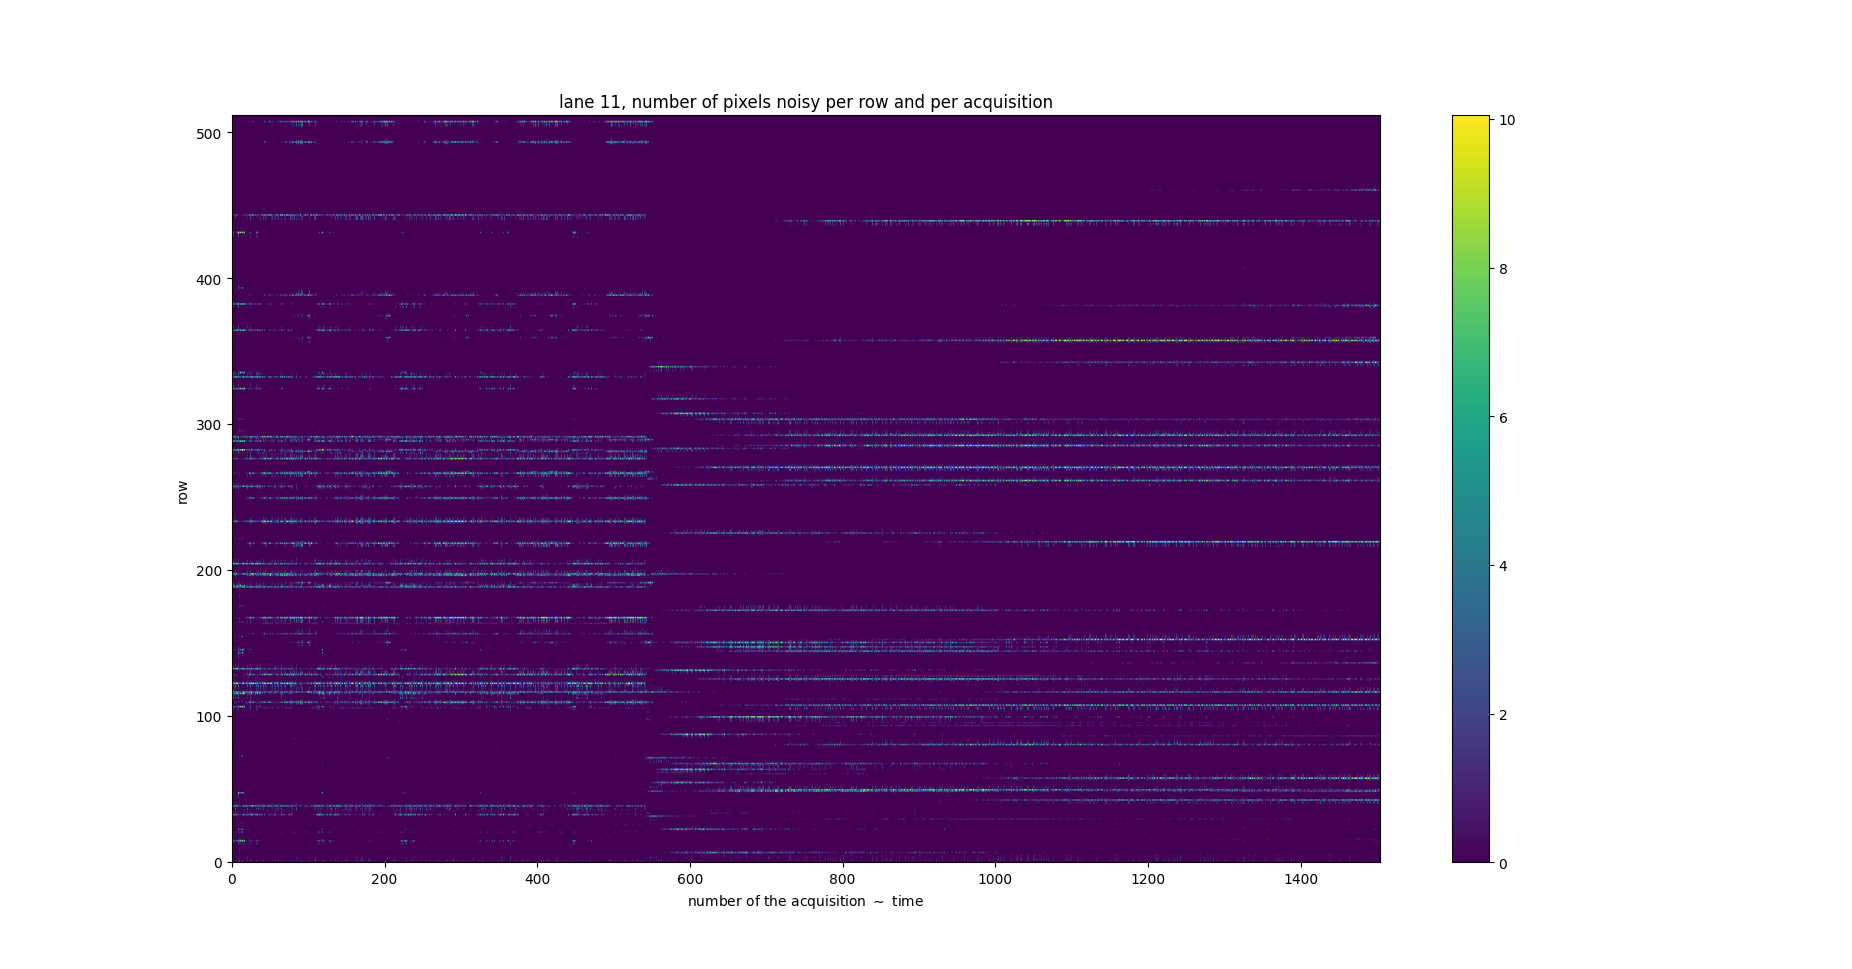
\includegraphics[width=.95\linewidth]{figures/charaterization/ARCADIA/pixel_per_row_per_acq_11_60.png}
        \caption{Noise in the front end circuit depending on the bias road across the matrix was recorded. }
        \label{fig:ARCADIA_threshold}
    \end{figure}

    %   Non ero entrata in dettaglio a proposito del baco perché non mi sembrava rilevante, ma non ho nessun problema a farlo ora. Durante la seconda sottomissione ci siamo accorti che il segnale che abilita i drivers LVDS delle sezioni aveva polarità sbagliata. I drivers LVDS sono quei circuiti che pilotano i dati verso il mondo esterno e avere un enable di polarità errata significa che i drivers risultano sempre spenti durante l'acquisizione. Quindi in pratica il chip funziona, ma non è in grado di trasmettere nulla all'esterno. Il segnale di enable viene controllato internamente al chip dalla logica di periferia e non è direttamente accessibile da fuori. Fortunatamente le linee di metallo che pilotano il suddetto segnale sono in una regione del chip poco densa, cioè senza altro metallo sopra e attorno. E' stato quindi possibile intervenire con un fascio di ioni focalizzato per andare a scavare nelle regioni di interesse fino ad accedere ai segnali di enable. Abbiamo quindi tagliato la connessione interna e cortocircuitato l'enable  al valore di tensione corretto.  Nel minid 2 questa correzione è stata fatta sul chip ed è l'unica modifica rispetto alla prima sottomissione.


    % Threshold (electrons):
    %   VCASN  |   e-
    %----------------
    %      0    | fe off
    %      1    |  835
    %      4    |  625
    %      7    |  475
    %      10   |  400
    %      16   |  360
    %      25   |  290
    %      31   |  220
    %      37   |  145
    %      ...
    %      63   |  min

    We received then another chip, a minid2, that is a "mini demonstrator" from the second submission. The two chips have the same charateristics but the minid2 is smaller than the MD1, in particular it only have 32$\times$512 pixels, instead of 512$\times$512.  
    \red{scrivi il problema della prima sottomissione.}


    An exhaustive characterization and testing of the new chip have been going on in the clean room on the INFN, and I am going to show here only some preliminary results.
    Up to now we used the injection circuit in order to make a threshold scan on a few pixels: differently from the TJ-Monopix1's charaterization where we performed a scan changing the injection charge of the pulse, with the minid2 we have instead changed the threshold (whose register is VCASN) keeping the charge of the pulse fixed.
    For each threshold we inject 100 pulses of amplitude \SI{10}{\us}. The dependece of the efficiency on the threshold for two pixels is shown in figure \ref{fig:ARCADIA_threshold}.  
    \begin{figure}[h!]
        \centering
        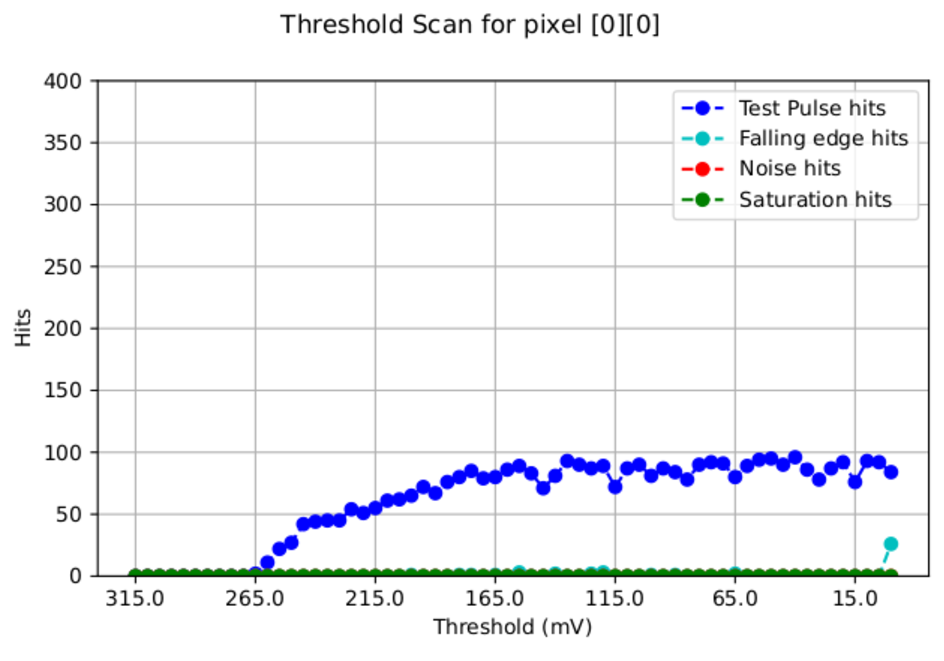
\includegraphics[width=.7\linewidth]{figures/charaterization/ARCADIA/threshold_0_0.pdf}
        \caption{}
        \label{fig:ARCADIA_threshold}
    \end{figure} 
    
    \red{Anche se il comportamento è globalmente ragionevole, con l'efficienza che sale quando si abbassa la soglia, viene il sospetto che non stiamo polarizzando bene il sensore e il FE dato che anche raggiunto i centi conteggi, si hanno delle fluttuazioni intorno a questo valore. Inoltre notiamo che abbassando ulteriormente la soglia si osserva un aumento delle hit, dovuto al fatto che si inizia a triggerare sul rumore. }

    \red{commenta sul fatto che non è stabile anche molto sopra la soglia. Forse è dovuto al bias? oppure l 'impulso ha qualche problema (non abbiamo settato la durata ecc..)? Che valore ha in elettroni?}

    Substantial differences have been observed in both the efficiency and the threshold among the sections, with VCASN=\SI{40}{DAC}; this suggests that with this particular FE configuration there is a big threshold dispersion on the matrix.  
    The hitmap of an acquisition with the Fe55 source is shown in figure \ref{fig:ARCADIA_Fe55}: the whole MD1 matrix with only the bottom region (32 rows) working is represented in (a), while in (b) there is a zoomed hitmap. The rate seen within the region 8 (green region in the figure (a)) is compatible with the rate of the same radioactive source measured with TJ-Monopix1, that it $\sim$\SI{3.3}{kHz}. 
    \begin{figure}[h!]
        \centering
        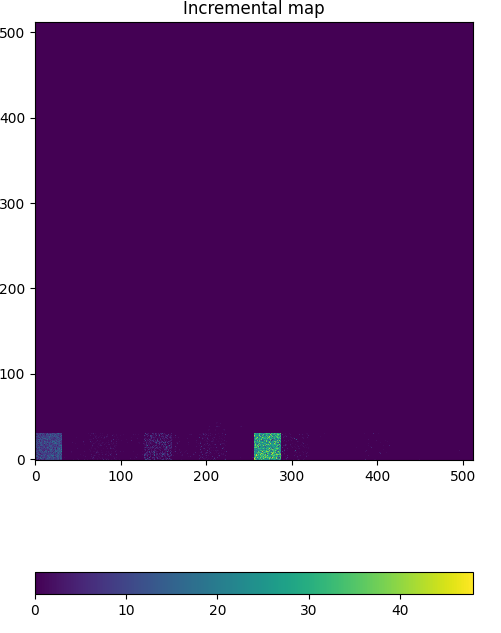
\includegraphics[width=.49\linewidth]{figures/charaterization/ARCADIA/Fe55_5min30s.png}
        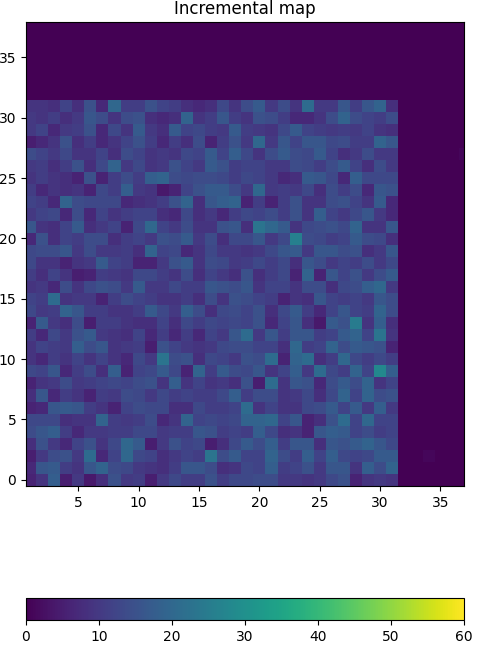
\includegraphics[width=.47\linewidth]{figures/charaterization/ARCADIA/Fe55_6min30s.png}
        \caption{Fe55 acquisition with VCASN=\SI{40}{DAC}. (a) All the matrix 512$\times$512 is plotted even if the minid2 has only the rows in range 0-32. (b) A zoom on the first section (col 0-32).   }
        \label{fig:ARCADIA_Fe55}
    \end{figure}  
    Looking to the Sr90 acquisitions (fig.\ref{fig:ARCADIA_Sr90}) many clusters and tracks can be immidiately distiguished, confirming what observed with TJ-Monopix1. 
    \begin{figure}[h!]
        \centering
        %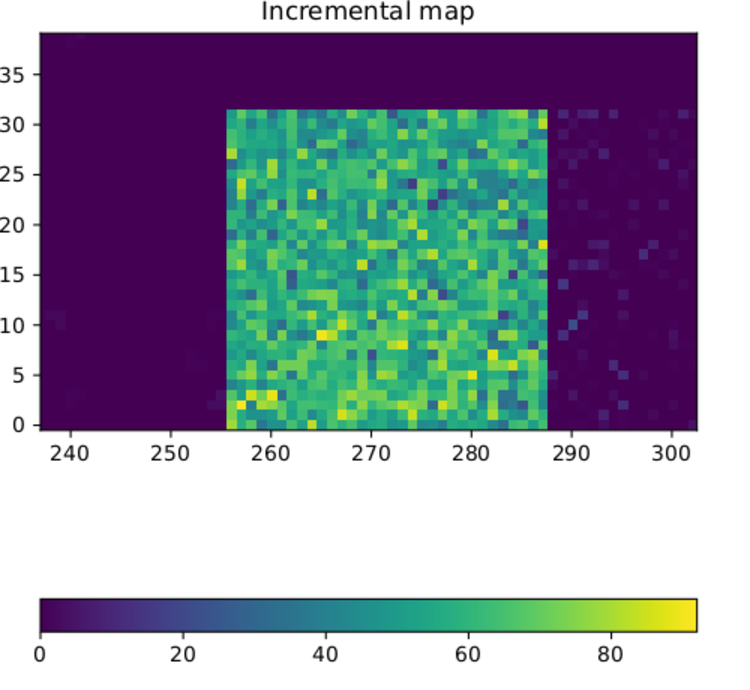
\includegraphics[width=.49\linewidth]{figures/charaterization/ARCADIA/Fe55_9min.pdf}
        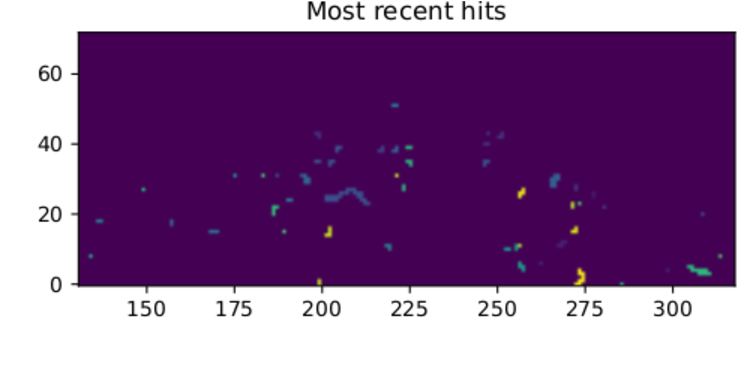
\includegraphics[width=.7\linewidth]{figures/charaterization/ARCADIA/Sr90_2min.pdf}
        \caption{Sr90 acquisition with VCASN=\SI{40}{DAC}. The different colours are related with the time of arrival of the hits: in yellow the most recent hits, while in blue the old ones.}
        \label{fig:ARCADIA_Sr90}
    \end{figure}  

    %test_play_wip.py,
    % example/test_initialization.py
    %example/test_play_triggered_wip.py 




